\documentclass[12pt,a4paper]{article}
\usepackage[a4paper, margin=0.8in, headheight=14pt]{geometry}
\usepackage{fontspec}
\usepackage{unicode-math}
\setmainfont{TeX Gyre Pagella}
\setmonofont[Scale=0.88]{TeX Gyre Cursor}
\setmathfont{Latin Modern Math}
\usepackage{xcolor}
\usepackage{colortbl}
\usepackage{titlesec}
\usepackage{enumitem}
\usepackage{tabularx}
\usepackage{booktabs}
\usepackage{array}
\usepackage{amsmath}
\usepackage{tikz}
\usetikzlibrary{shapes.geometric, arrows.meta, positioning, calc, fit, decorations.pathreplacing, decorations.pathmorphing, patterns}
\usepackage[american]{circuitikz}
\usepackage{tcolorbox}
\tcbuselibrary{skins, breakable}
\usepackage{hyperref}
\usepackage{fancyhdr}
\usepackage{graphicx}
\usepackage{microtype}
\hyphenpenalty=10000
\exhyphenpenalty=10000
\sloppy
\usepackage{caption}
\usepackage{setspace}
\usepackage{multirow}
\usepackage{tocloft}
\newcommand{\Q}[1]{\textbf{#1}\par\noindent\ignorespaces}
\definecolor{myred}{RGB}{196,30,58}
\definecolor{mydark}{RGB}{30,30,50}
\definecolor{mygreen}{RGB}{14,120,80}
\definecolor{myteal}{RGB}{0,130,140}
\definecolor{myamber}{RGB}{180,100,0}
\definecolor{mypurple}{RGB}{100,30,160}
\definecolor{mygray}{RGB}{246,247,249}
\definecolor{mgframe}{RGB}{180,185,200}
\definecolor{watermark}{RGB}{145,150,170}
\definecolor{hdrred}{RGB}{250,232,235}
\definecolor{hdrgreen}{RGB}{220,244,233}
\definecolor{hdrteal}{RGB}{220,242,244}
\definecolor{hdramber}{RGB}{253,242,215}
\definecolor{hdrpurple}{RGB}{238,228,255}

\titleformat{\section}{\large\bfseries\color{myred}}{\thesection.}{0.5em}{}[\vspace{1pt}{\color{myred}\rule{\linewidth}{0.8pt}}]
\titleformat{\subsection}{\normalsize\bfseries\color{myteal}}{\thesubsection}{0.5em}{}
\titlespacing*{\section}{0pt}{18pt}{7pt}
\titlespacing*{\subsection}{0pt}{11pt}{4pt}
\setlength{\parindent}{0pt}
\setlength{\parskip}{4pt}
\renewcommand{\cfttoctitlefont}{\large\bfseries\color{myred}}
\renewcommand{\cftaftertoctitle}{\par\noindent{\color{myred}\rule{\linewidth}{0.8pt}}}
\setlength{\cftbeforetoctitleskip}{0pt}
\setlength{\cftaftertoctitleskip}{6pt}
\renewcommand{\cftsecfont}{\normalsize\bfseries\color{mydark}}
\renewcommand{\cftsecpagefont}{\normalsize\bfseries\color{mydark}}
\renewcommand{\cftsecleader}{\cftdotfill{\cftdotsep}}
\setlength{\cftbeforesecskip}{7pt}
\renewcommand{\cftsubsecfont}{\small\color{mydark}}
\renewcommand{\cftsubsecpagefont}{\small\color{mydark}}
\setlength{\cftbeforesubsecskip}{3pt}
\setlength{\cftsubsecindent}{1.4em}
\renewcommand{\cftpartfont}{\normalsize\bfseries\color{myteal}}
\renewcommand{\cftpartpagefont}{\normalsize\bfseries\color{myteal}}
\setlength{\cftbeforepartskip}{14pt}
\renewcommand{\arraystretch}{1.45}
\setlength{\tabcolsep}{6pt}
\arrayrulecolor{mydark}
\newcolumntype{B}[1]{>{\small\bfseries\raggedright\arraybackslash}m{#1}}
\newcolumntype{C}[1]{>{\centering\arraybackslash}m{#1}}
\newcolumntype{Y}{>{\small\raggedright\arraybackslash}X}
\renewcommand{\tabularxcolumn}[1]{m{#1}}
\newcommand{\currmodule}{Module 1}
\pagestyle{fancy}
\fancyhf{}
\fancyhead[L]{\small\color{myred}\textbf{PE-EC801C}\;\color{mydark}--- Error Correcting Codes}
\fancyhead[R]{\small\color{myteal}\textbf{\currmodule\ Notes}}
\fancyfoot[C]{\small\color{mydark}\thepage}
\fancyfoot[R]{\small\color{watermark}\textit{\copyright\ Biraj}}
\renewcommand{\headrulewidth}{0.5pt}
\renewcommand{\footrulewidth}{0.3pt}

\hypersetup{colorlinks=true, linkcolor=myteal, urlcolor=myteal,
  pdfauthor={Biraj Sarkar},
  pdftitle={PE-EC801C --- Combined Notes}}

\tcbset{
  tikzbox/.style={
    colback=mygray, colframe=mgframe, boxrule=0.6pt, arc=4pt,
    left=8pt, right=8pt, top=6pt, bottom=6pt,
    colbacktitle=mgframe, coltitle=mydark,
    fonttitle=\small\bfseries
  },
  defbox/.style={
    colback=hdrgreen, colframe=mygreen, boxrule=0.8pt, arc=4pt,
    left=9pt, right=9pt, top=6pt, bottom=6pt,
    colbacktitle=mygreen, coltitle=white,
    fonttitle=\small\bfseries
  },
  formulabox/.style={
    colback=hdrteal, colframe=myteal, boxrule=0.8pt, arc=4pt,
    left=9pt, right=9pt, top=7pt, bottom=7pt,
    colbacktitle=myteal, coltitle=white,
    fonttitle=\small\bfseries
  },
  examplebox/.style={
    colback=hdramber, colframe=myamber, boxrule=0.8pt, arc=4pt,
    left=9pt, right=9pt, top=6pt, bottom=6pt,
    colbacktitle=myamber, coltitle=white,
    fonttitle=\small\bfseries
  },
  masonbox/.style={
    colback=hdrpurple, colframe=mypurple, boxrule=0.8pt, arc=4pt,
    left=9pt, right=9pt, top=6pt, bottom=6pt,
    colbacktitle=mypurple, coltitle=white,
    fonttitle=\small\bfseries
  },
  exambox/.style={
    colback=hdrpurple, colframe=mypurple, boxrule=1pt, arc=5pt,
    left=10pt, right=10pt, top=8pt, bottom=8pt,
    colbacktitle=mypurple, coltitle=white,
    fonttitle=\bfseries,
    breakable, title after break={\textbf{Frequently Asked / Viva Questions (contd.)}}}
}
\tcbset{breakable}
\tcbset{after={\color{black}}}

\tikzset{
  block/.style={rectangle, draw=myteal, fill=hdrteal,
    text width=2.4cm, align=center, minimum height=0.95cm,
    font=\small, rounded corners=3pt, line width=0.7pt},
  redblock/.style={rectangle, draw=myred, fill=hdrred,
    text width=2.4cm, align=center, minimum height=0.95cm,
    font=\small, rounded corners=3pt, line width=0.7pt},
  sumjunc/.style={circle, draw=myamber, fill=hdramber,
    minimum size=0.62cm, font=\small, line width=0.8pt},
  snode/.style={circle, draw=mypurple, fill=hdrpurple,
    minimum size=0.55cm, font=\footnotesize, line width=0.7pt},
  arrow/.style={-Stealth, thick, color=mydark},
  redarrow/.style={-Stealth, thick, color=myred},
  line/.style={thick, color=mydark},
  reg/.style={rectangle, draw=myteal, fill=hdrteal,
    minimum width=0.85cm, minimum height=0.85cm, align=center,
    font=\small\bfseries, line width=0.7pt},
  adder/.style={circle, draw=myamber, fill=hdramber,
    minimum size=0.45cm, font=\small\bfseries, line width=0.8pt, inner sep=0pt},
  mult/.style={circle, draw=mypurple, fill=hdrpurple,
    minimum size=0.45cm, font=\small, line width=0.7pt, inner sep=0pt},
  card/.style={rectangle, draw=mgframe, fill=white,
    text width=3.8cm, align=center, minimum height=0.9cm,
    font=\small\bfseries, rounded corners=6pt, line width=0.8pt},
  stepnode/.style={rectangle, draw=myteal, fill=hdrteal,
    text width=3.4cm, align=center, minimum height=1.0cm,
    font=\small\bfseries, rounded corners=4pt, line width=0.8pt},
  flowarrow/.style={-Stealth, thick, color=mydark},
  state/.style={circle, draw=myteal, fill=hdrteal,
    minimum size=0.9cm, font=\small\bfseries, line width=0.8pt},
  trellisnode/.style={circle, fill=mydark, inner sep=1.5pt}
}

\newcommand{\modulestart}[2]{%
  \clearpage
  \renewcommand{\currmodule}{Module #1}%
  \renewcommand{\theHsection}{mod#1.\arabic{section}}%
  \renewcommand{\theHsubsection}{\theHsection.\arabic{subsection}}%
  \renewcommand{\theHsubsubsection}{\theHsubsection.\arabic{subsubsection}}%
  \phantomsection
  \addcontentsline{toc}{part}{Module #1: #2}%
  \setcounter{section}{0}%
  \begin{center}
    \vspace*{1.0cm}
    {\Huge\bfseries\color{myred} Module #1}\\[10pt]
    {\Large\bfseries\color{mydark} #2}\\[10pt]
    {\color{myred}\rule{0.55\linewidth}{1.2pt}}
  \end{center}
  \vspace{14pt}
}
\begin{document}

\thispagestyle{empty}
\vspace*{1.0cm}
\begin{center}
  {\Huge\bfseries\color{myred} PE-EC801C}\\[10pt]
  {\LARGE\bfseries\color{mydark} Error Correcting Codes}\\[20pt]
  {\color{myred}\rule{0.7\linewidth}{1.5pt}}\\[18pt]
  {\Large\color{myteal}\textbf{Combined Module Notes}}\\[8pt]
  {\large\color{mydark} Modules 1 -- 5}\\[40pt]
  {\normalsize\color{mydark} Semester VIII \quad$\bullet$\quad 3L:0T:0P \quad$\bullet$\quad 3 Credits}\\[12pt]
  {\normalsize\color{mydark} CGEC \;$|$\; B.Tech ECE (2023--27)}\\[6pt]
  {\normalsize\color{mydark}\textit{Biraj Sarkar}}
\end{center}
\vspace{1.0cm}
\begin{center}
  \begin{tcolorbox}[colback=mygray, colframe=mgframe, boxrule=0.5pt, arc=3pt, width=0.85\linewidth]
    \centering\small\color{mydark}
    \textbf{Disclaimer / Study Guide Notice:}\\
    These are condensed \textbf{Short Notes} focusing on core theory, key formulas, block/circuit diagrams, and standard viva Q\&As for university exam revision. Exhaustive numerical practice problems and derivation edge cases are not covered. This serves as a quick-revision reference guide for students.
  \end{tcolorbox}
\end{center}
\vfill
\begin{center}{\small\color{watermark}\textit{Exam-Ready Notes}}\end{center}
\clearpage

\hypersetup{linkcolor=mydark}
\tableofcontents
\hypersetup{linkcolor=myteal}
\clearpage

% -- Module 1 -----------------------------------------------------------------
\modulestart{1}{Introduction to Block Coding}

\section{Introduction to Block Coding}
% ===============================================================================

Error control coding is a technique used to detect and correct transmission errors introduced by noisy communication channels. In \textbf{block coding}, a stream of information bits is partitioned into blocks of size $k$. The channel encoder maps each $k$-bit message block into a larger $n$-bit codeword by adding $n-k$ redundant parity-check bits.

\begin{tcolorbox}[defbox, title={\textbf{Key Coding Definitions}}]
\begin{itemize}[leftmargin=*, itemsep=3pt, topsep=0pt]
  \item \textbf{Code Word ($c$):} The output block of the channel encoder consisting of $n$ bits.
  \item \textbf{Block Length ($n$):} The total number of bits in a codeword.
  \item \textbf{Message Length ($k$):} The number of actual information bits in the block.
  \item \textbf{Redundancy ($n-k$):} The number of check bits added for error detection/correction.
  \item \textbf{Code Rate ($R$):} The ratio of information bits to total bits, representing transmission efficiency:
    \[ R = \frac{k}{n} \]
\end{itemize}
\end{tcolorbox}

\subsection{Vector Space Structure of Codewords}
The set of all binary $n$-tuples forms a vector space $V_n$ over the binary Galois Field $\text{GF}(2) = \{0, 1\}$. There are $2^n$ possible vectors in $V_n$. A binary block code $C$ of length $n$ with $2^k$ codewords is a subset of $V_n$. If $C$ is a vector subspace of $V_n$, it is called a \textbf{linear block code}. This algebraic structure implies that the sum (modulo-2 addition) of any two codewords in $C$ is also a valid codeword in $C$:
\[ \forall c_1, c_2 \in C \implies c_1 \oplus c_2 \in C \]

\subsection{Weight and Distance Metrics}
Error correction capability depends on the distance between codewords. We define the following metrics over the binary field:
\begin{tcolorbox}[defbox, title={\textbf{Weight and Distance Definitions}}]
\begin{itemize}[leftmargin=*, itemsep=3pt, topsep=0pt]
  \item \textbf{Hamming Weight ($w(x)$):} The number of non-zero elements in a vector $x \in V_n$.
  \item \textbf{Hamming Distance ($d(x, y)$):} The number of positions in which two vectors $x$ and $y$ differ. This is equivalent to the weight of their modulo-2 sum:
    \[ d(x, y) = w(x \oplus y) \]
  \item \textbf{Minimum Distance ($d_{min}$):} The smallest Hamming distance between any two distinct codewords in the code $C$:
    \[ d_{min} = \min \{ d(c_i, c_j) \mid c_i, c_j \in C, \, c_i \neq c_j \} \]
\end{itemize}
\end{tcolorbox}

For any linear block code, the minimum distance is equal to the minimum weight of any non-zero codeword in the code:
\[ d_{min} = \min \{ w(c) \mid c \in C, \, c \neq 0 \} \]

\subsection{Error Detection and Correction Capabilities}
\begin{tcolorbox}[formulabox, title={\textbf{Error Bounds}}]
Let $d_{min}$ be the minimum distance of a block code $C$.
\begin{enumerate}[leftmargin=*, itemsep=3pt, topsep=0pt]
  \item \textbf{Error Detection:} A code can detect up to $t_d$ random errors per codeword if:
    \[ d_{min} \ge t_d + 1 \]
  \item \textbf{Error Correction:} A code can correct up to $t_c$ random errors per codeword if:
    \[ d_{min} \ge 2t_c + 1 \implies t_c = \left\lfloor \frac{d_{min} - 1}{2} \right\rfloor \]
\end{enumerate}
\end{tcolorbox}

% ===============================================================================
\section{Systematic Linear Block Codes}
% ===============================================================================

A block code is \textbf{systematic} if the message bits appear unaltered at the beginning (or end) of the codeword, followed by the parity-check bits. A systematic codeword vector $c$ can be partitioned as:
\[ c = [m_0, m_1, \dots, m_{k-1}, p_0, p_1, \dots, p_{n-k-1}] = [m \mid p] \]

\subsection{The Generator Matrix \texorpdfstring{$G$}{G}}
The encoding process is defined by a $k \times n$ matrix called the \textbf{Generator Matrix} $G$. Every codeword is generated by multiplying the $k$-bit message vector $m$ by $G$:
\[ c = m \cdot G \]
For a systematic linear block code, $G$ is structured as:
\[ G = [I_k \mid P] \]
where $I_k$ is the $k \times k$ identity matrix (generating the message part) and $P$ is a $k \times (n-k)$ parity-check coefficient matrix (generating the redundant part).
\[ G = \begin{bmatrix}
  1 & 0 & \dots & 0 & p_{0,0} & p_{0,1} & \dots & p_{0,n-k-1} \\
  0 & 1 & \dots & 0 & p_{1,0} & p_{1,1} & \dots & p_{1,n-k-1} \\
  \vdots & \vdots & \ddots & \vdots & \vdots & \vdots & \ddots & \vdots \\
  0 & 0 & \dots & 1 & p_{k-1,0} & p_{k-1,1} & \dots & p_{k-1,n-k-1}
\end{bmatrix} \]
The parity bits are computed by:
\[ p_j = \sum_{i=0}^{k-1} m_i p_{i,j} \pmod 2 \]

\subsection{The Parity Check Matrix \texorpdfstring{$H$}{H}}
The parity check matrix $H$ is an $(n-k) \times n$ matrix used to verify if a received vector is a valid codeword. By definition, any valid codeword $c \in C$ must satisfy the orthogonal relation:
\[ c \cdot H^T = \mathbf{0} \]
For a systematic code where $G = [I_k \mid P]$, the parity check matrix is:
\[ H = [P^T \mid I_{n-k}] \]
where $P^T$ is the transpose of the parity matrix and $I_{n-k}$ is the $(n-k) \times (n-k)$ identity matrix.

\begin{tcolorbox}[examplebox, title={\textbf{Verification of Orthogonality}}]
Let us verify the relationship $G \cdot H^T = \mathbf{0}$:
\[ G \cdot H^T = [I_k \mid P] \begin{bmatrix} P \\ I_{n-k} \end{bmatrix} = I_k \cdot P \oplus P \cdot I_{n-k} = P \oplus P = \mathbf{0} \pmod 2 \]
Since $c = m \cdot G$, we have:
\[ c \cdot H^T = (m \cdot G) \cdot H^T = m \cdot (G \cdot H^T) = m \cdot \mathbf{0} = \mathbf{0} \]
This confirms that the parity check matrix successfully screens for codewords.
\end{tcolorbox}

% ===============================================================================
\section{Optimum Decoding for the Binary Symmetric Channel}
% ===============================================================================

Let $c$ be the transmitted codeword and $r = [r_0, r_1, \dots, r_{n-1}]$ be the received vector. Due to channel noise, $r = c \oplus e$, where $e = [e_0, e_1, \dots, e_{n-1}]$ is the binary error vector ($e_i = 1$ indicates a bit inversion error at position $i$).

\subsection{The Binary Symmetric Channel (BSC)}
The BSC is a discrete memoryless channel with binary input, binary output, and a crossover probability $p$ ($p < 0.5$).

\begin{tcolorbox}[tikzbox, title={Binary Symmetric Channel Model}]
\centering
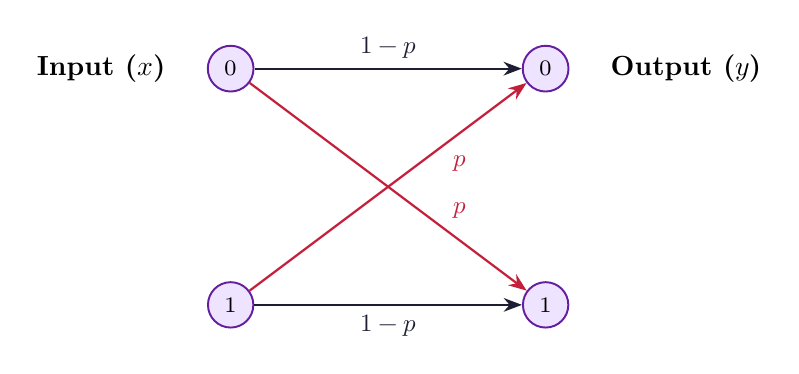
\begin{tikzpicture}[node distance=2.2cm and 3.2cm]
  \node[snode] (x0) at (0, 1.5) {$0$};
  \node[snode] (x1) at (0, -1.5) {$1$};
  \node[snode] (y0) at (4, 1.5) {$0$};
  \node[snode] (y1) at (4, -1.5) {$1$};

  \draw[arrow] (x0) -- node[above, pos=0.5]{\small $1-p$} (y0);
  \draw[arrow] (x1) -- node[below, pos=0.5]{\small $1-p$} (y1);
  \draw[redarrow] (x0) -- node[above right, pos=0.7]{\small $p$} (y1);
  \draw[redarrow] (x1) -- node[below right, pos=0.7]{\small $p$} (y0);
  
  \node[left=0.4cm of x0] {\textbf{Input ($x$)}};
  \node[right=0.4cm of y0] {\textbf{Output ($y$)}};
\end{tikzpicture}
\end{tcolorbox}

\subsection{Maximum Likelihood (ML) Decoding}
An optimum decoder minimizes the probability of decoding error. The maximum likelihood decoding rule selects the codeword $c^{(i)}$ that maximizes the conditional probability $P(r \mid c^{(i)})$:
\[ P(r \mid c^{(i)}) = p^{d(r, c^{(i)})} (1-p)^{n-d(r, c^{(i)})} \]
Since $p < 0.5 \implies 1-p > p$, we can rewrite this by taking the logarithm:
\[ \ln P(r \mid c^{(i)}) = d(r, c^{(i)}) \ln \left(\frac{p}{1-p}\right) + n \ln(1-p) \]
Since $\ln(p/(1-p)) < 0$ for $p < 0.5$, maximizing $P(r \mid c^{(i)})$ is mathematically equivalent to minimizing the Hamming distance:
\[ \text{ML Decoding Rule:} \quad \text{Choose } c \in C \text{ that minimizes } d(r, c) \]
Thus, over a BSC, Maximum Likelihood decoding simplifies to \textbf{minimum distance decoding}.

% ===============================================================================
\section{Syndrome Decoding on Symmetric Channels}
% ===============================================================================

Instead of calculating the distance from $r$ to all $2^k$ codewords, we can use the parity check matrix to compute a \textbf{Syndrome} vector $S$.

\begin{tcolorbox}[defbox, title={\textbf{The Syndrome}}]
The syndrome of a received vector $r$ is defined as:
\[ S = r \cdot H^T \]
\end{tcolorbox}

\subsection{Properties of the Syndrome}
\begin{enumerate}[label=\textbf{\arabic*.}, leftmargin=*, itemsep=3pt]
  \item $S = \mathbf{0}$ if and only if $r$ is a valid codeword.
  \item The syndrome depends \textbf{only on the error pattern} $e$, not on the transmitted codeword $c$:
    \[ S = r \cdot H^T = (c \oplus e) \cdot H^T = (c \cdot H^T) \oplus (e \cdot H^T) = \mathbf{0} \oplus (e \cdot H^T) = e \cdot H^T \]
  \item Two received vectors $r_1$ and $r_2$ have the same syndrome if and only if they differ by a valid codeword.
\end{enumerate}

\subsection{The Standard Array and Coset Leaders}
A standard array partitions the $2^n$ possible received vectors into a table of $2^{n-k}$ rows (called \textbf{cosets}) and $2^k$ columns.

\textbf{Standard Array Construction Algorithm:}\par\noindent
\begin{enumerate}[leftmargin=*, itemsep=3pt]
  \item Place all $2^k$ valid codewords in the first row, starting with the all-zero codeword $c_0 = \mathbf{0}$ on the far left.
  \item From the remaining unused vectors in $V_n$, choose a vector $e_1$ of minimum weight. Place it in the first column of the second row. This vector is the \textbf{coset leader}.
  \item Fill the second row by adding the coset leader $e_1$ to each codeword: $e_1 \oplus c_i$.
  \item Repeat this process: choose a minimum weight unused vector $e_j$ as the next coset leader, and fill the row with $e_j \oplus c_i$, until all $2^n$ vectors are placed.
\end{enumerate}

\begin{tcolorbox}[tikzbox, title={Standard Array Layout}]
{\renewcommand{\arraystretch}{1.5}%
\begin{tabularx}{\linewidth}{|>{\centering\arraybackslash}X|>{\centering\arraybackslash}X|>{\centering\arraybackslash}X|>{\centering\arraybackslash}X|>{\centering\arraybackslash}X|}
\hline
\textbf{Coset Leader ($e_j$)} & \textbf{Codeword $c_0=\mathbf{0}$} & \textbf{Codeword $c_1$} & \dots & \textbf{Codeword $c_{2^k-1}$} \\
\hline
$e_0 = \mathbf{0}$ & $\mathbf{0}$ & $c_1$ & \dots & $c_{2^k-1}$ \\
\hline
$e_1$ & $e_1$ & $e_1 \oplus c_1$ & \dots & $e_1 \oplus c_{2^k-1}$ \\
\hline
\vdots & \vdots & \vdots & \ddots & \vdots \\
\hline
$e_{2^{n-k}-1}$ & $e_{2^{n-k}-1}$ & $e_{2^{n-k}-1} \oplus c_1$ & \dots & $e_{2^{n-k}-1} \oplus c_{2^k-1}$ \\
\hline
\end{tabularx}}
\end{tcolorbox}

Each row (coset) corresponds to a unique syndrome. The coset leader is the \textbf{most likely error pattern} for that syndrome because it has the minimum weight in its coset.

\subsection{Syndrome Decoding Algorithm}
\begin{tcolorbox}[formulabox, title={\textbf{Syndrome Decoding Steps}}]
\begin{enumerate}[label=\textbf{Step \arabic*:}, leftmargin=2.0cm, itemsep=2pt]
  \item Compute the syndrome of the received vector: $S = r \cdot H^T$.
  \item Find the coset leader $e$ that matches this syndrome: $e \cdot H^T = S$.
  \item Correct the received vector to obtain the decoded codeword:
    \[ \hat{c} = r \oplus e \]
\end{enumerate}
\end{tcolorbox}

% ===============================================================================
\section{Hamming Codes}
% ===============================================================================

Hamming codes are a class of single-error-correcting linear block codes. For any integer $m \ge 2$, there exists a Hamming code with the following parameters:

\begin{tcolorbox}[defbox, title={\textbf{Hamming Code Parameters}}]
\begin{itemize}[leftmargin=*, itemsep=3pt, topsep=0pt]
  \item \textbf{Parity bits:} $n - k = m$
  \item \textbf{Code length:} $n = 2^m - 1$
  \item \textbf{Message length:} $k = 2^m - 1 - m$
  \item \textbf{Minimum distance:} $d_{min} = 3$
  \item \textbf{Error Correction:} Corrects all single errors ($t_c = 1$).
\end{itemize}
\end{tcolorbox}

\subsection{Structure of the Parity Check Matrix}
The parity check matrix $H$ of a Hamming code has $m$ rows and $2^m - 1$ columns. The columns of $H$ consist of all possible non-zero binary $m$-tuples, arranged in any order. In a systematic Hamming code:
\[ H = [P^T \mid I_m] \]
where the columns of $P^T$ consist of all non-zero binary $m$-tuples with weight $\ge 2$.

\subsection{Decoding of Hamming Codes}
When a single error occurs at position $i$, the received vector is $r = c \oplus e_i$, where $e_i$ has a $1$ at index $i$ and zeros elsewhere. The syndrome is:
\[ S = r \cdot H^T = (c \oplus e_i) \cdot H^T = e_i \cdot H^T = h_i^T \]
where $h_i^T$ is the transpose of the $i$-th column of $H$. Therefore, the syndrome $S$ is \textbf{identical to the column of $H$ corresponding to the error location}. If the columns of $H$ are arranged in order of their decimal equivalents, $S$ directly represents the index of the corrupted bit in binary.

% ===============================================================================
\section{Weight Enumerators and McWilliams Identities}
% ===============================================================================

The performance of a block code is determined by its \textbf{Weight Distribution}. Let $A_i$ be the number of codewords in $C$ with Hamming weight $i$. The set $\{A_0, A_1, \dots, A_n\}$ is the weight spectrum of the code.

\subsection{The Weight Enumerator Polynomial}
The weight distribution can be expressed as a polynomial:
\begin{tcolorbox}[defbox, title={\textbf{Weight Enumerator Polynomial}}]
\[ A(z) = \sum_{i=0}^n A_i z^i = A_0 + A_1 z + A_2 z^2 + \dots + A_n z^n \]
where $A_0 = 1$ (the all-zero codeword).
\end{tcolorbox}

\subsection{The McWilliams Identities}
The McWilliams identities relate the weight enumerator polynomial $A(z)$ of a linear block code $C$ of length $n$ to the weight enumerator polynomial $A^\perp(z)$ of its \textbf{dual code} $C^\perp$. The dual code $C^\perp$ is the set of all vectors orthogonal to every codeword in $C$, having dimension $n-k$ and generator matrix $H$.

\begin{tcolorbox}[formulabox, title={\textbf{McWilliams Identity Theorem}}]
For a binary $[n, k]$ linear code $C$ with weight enumerator $A(z)$ and dual code $C^\perp$ with weight enumerator $A^\perp(z)$:
\[ A^\perp(z) = \frac{1}{2^k} (1+z)^n A\left( \frac{1-z}{1+z} \right) \]
Alternatively, writing as a homogeneous polynomial in two variables $x$ and $y$:
\[ W_{C^\perp}(x, y) = \frac{1}{2^k} W_C(x+y, x-y) \]
\end{tcolorbox}
This identity is useful because it allows us to find the weight distribution of a code with large $k$ by analyzing its dual code which has a smaller dimension $n-k$ (e.g., finding the weight distribution of a $(127, 120)$ Hamming code by analyzing its $(127, 7)$ dual code).

% ===============================================================================
\section{Perfect Codes}
% ===============================================================================

For any block code correcting up to $t$ errors, the sphere of radius $t$ centered around each codeword must be disjoint. The total volume of these spheres cannot exceed the size of the vector space $2^n$.

\subsection{The Hamming Bound (Sphere-Packing Bound)}
The number of vectors in a sphere of radius $t$ in $V_n$ is:
\[ V(n, t) = \sum_{i=0}^t \binom{n}{i} \]
For $2^k$ codewords, we must have:
\[ 2^k \sum_{i=0}^t \binom{n}{i} \le 2^n \implies \sum_{i=0}^t \binom{n}{i} \le 2^{n-k} \]

\begin{tcolorbox}[defbox, title={\textbf{Perfect Code Definition}}]
A block code is a \textbf{Perfect Code} if it satisfies the Hamming bound with equality:
\[ 2^k \sum_{i=0}^t \binom{n}{i} = 2^n \]
In a perfect code, every vector in the space $V_n$ lies in exactly one sphere of radius $t$ around a codeword. There are no "wasted" vectors that cannot be corrected.
\end{tcolorbox}

\subsection{Examples of Perfect Codes}
Only a few families of perfect codes exist:
\begin{enumerate}[label=\textbf{\arabic*.}, leftmargin=*, itemsep=3pt]
  \item \textbf{Single-Error-Correcting Hamming Codes ($t=1$):}
    Satisfy: $1 + n = 2^{n-k} \implies 1 + (2^m - 1) = 2^m \quad \checkmark$
  \item \textbf{The Binary Golay Code ($[23, 12, 7]$):}
    Corrects $t=3$ errors.
    \[ \sum_{i=0}^3 \binom{23}{i} = 1 + 23 + 253 + 1771 = 2048 = 2^{11} = 2^{23-12} \quad \checkmark \]
  \item \textbf{The Ternary Golay Code ($[11, 6, 5]$):}
    Defined over GF(3), corrects $t=2$ errors.
    \[ \sum_{i=0}^2 \binom{11}{i} 2^i = 1 + 11(2) + 55(4) = 1 + 22 + 220 = 243 = 3^5 = 3^{11-6} \quad \checkmark \]
  \item \textbf{Trivial Perfect Codes:} The whole space ($d_{min}=1$), and binary repetition codes of odd length $n$ ($d_{min}=n, t = (n-1)/2$).
\end{enumerate}

% ═══════════════════════════════════════════════════════════════════════════════
% QUICK REVISION PAGE
% ═══════════════════════════════════════════════════════════════════════════════
\newpage
\begin{center}
  {\large\bfseries\color{myred} Quick Revision --- Module 1}\\[3pt]
  {\small\color{mydark} Linear Block Codes $|$ PE-EC801C}
\end{center}
\noindent{\color{myred}\rule{\linewidth}{1.2pt}}
\vspace{4pt}

\begin{tcolorbox}[formulabox, title={\textbf{Key Formulas and Metrics at a Glance}}]
\renewcommand{\arraystretch}{1.35}
\begin{tabularx}{\linewidth}{B{5.0cm} X}
Code Rate & $R = k/n$ \\[4pt]
Hamming Distance & $d(x, y) = w(x \oplus y)$ \\[4pt]
Error Correction Limit & $t_c = \lfloor (d_{min}-1)/2 \rfloor$ \\[4pt]
Systematic Generator Matrix & $G = [I_k \mid P]$ \\[4pt]
Parity Check Matrix & $H = [P^T \mid I_{n-k}]$ \\[4pt]
Orthogonality Condition & $G \cdot H^T = \mathbf{0} \pmod 2$ and $c \cdot H^T = \mathbf{0}$ \\[4pt]
Syndrome Vector & $S = r \cdot H^T = e \cdot H^T$ \\[4pt]
Hamming Bound (Sphere-Packing) & $2^k \sum_{i=0}^t \binom{n}{i} \le 2^n$ \\[4pt]
McWilliams Identity & $A^\perp(z) = \frac{1}{2^k} (1+z)^n A\left( \frac{1-z}{1+z} \right)$ \\[4pt]
Hamming Code Parameters & Length $n = 2^m-1$, Info bits $k = 2^m-1-m$, $d_{min}=3$
\end{tabularx}
\end{tcolorbox}

\vspace{6pt}

\begin{tcolorbox}[defbox, title={\textbf{One-Line Definitions}}]
\begin{itemize}[leftmargin=*, itemsep=3pt, topsep=0pt]
  \item \textbf{Linear Block Code:} A code where the modulo-2 sum of any two codewords is also a valid codeword.
  \item \textbf{Minimum Distance ($d_{min}$):} The smallest Hamming distance between any two distinct codewords in a code.
  \item \textbf{Syndrome:} A vector calculated as $r \cdot H^T$ that indicates if errors occurred and helps locate them.
  \item \textbf{Coset Leader:} The vector with the smallest Hamming weight in a coset, representing the most likely error.
  \item \textbf{Hamming Code:} A class of perfect single-error-correcting codes with minimum distance $d_{min} = 3$.
  \item \textbf{Perfect Code:} A code that satisfies the Hamming (sphere-packing) bound with strict equality.
  \item \textbf{Dual Code ($C^\perp$):} The set of all vectors orthogonal to every codeword in the original code $C$.
  \item \textbf{Binary Symmetric Channel:} A binary input/output channel where bit-flip probability is equal for $0$ and $1$.
\end{itemize}
\end{tcolorbox}

\newpage

\begin{tcolorbox}[exambox, title={\textbf{Frequently Asked / Viva Questions}}]
\begin{enumerate}[topsep=0pt, label=\textbf{Q\arabic*.}, itemsep=5pt]
  \item \Q{What is the difference between systematic and non-systematic codes?}
    In systematic codes, the message bits are placed directly at the beginning or end of the codeword, making extraction trivial. In non-systematic codes, message and parity bits are interleaved or mathematically combined throughout the codeword.
  \item \Q{Prove that $d_{min} = w_{min}$ for linear block codes.}
    For linear block codes, if $c_1, c_2 \in C$ are codewords, then $c_1 \oplus c_2 = c_3 \in C$ is also a codeword. The distance is $d(c_1, c_2) = w(c_1 \oplus c_2) = w(c_3)$. Thus, minimizing distance between distinct codewords is equivalent to finding the minimum weight of non-zero codewords.
  \item \Q{What is the physical significance of the syndrome vector?}
    The syndrome represents the parity-check violations of the received vector. Because $S = e \cdot H^T$, it depends strictly on the channel error pattern, not on the transmitted data, allowing isolated error isolation.
  \item \Q{Explain the ML decoding criteria over a Binary Symmetric Channel.}
    Maximum Likelihood decoding selects the codeword that maximizes $P(r \mid c)$. On a BSC with crossover probability $p < 0.5$, this probability increases as the distance $d(r, c)$ decreases. Thus, ML decoding reduces to minimum Hamming distance decoding.
  \item \Q{Why are Hamming codes considered perfect codes?}
    Hamming codes have $d_{min}=3$, meaning they correct $t=1$ error. They satisfy the sphere-packing bound with equality since $\sum_{i=0}^1 \binom{n}{i} = 1 + n = 1 + 2^m - 1 = 2^m = 2^{n-k}$, leaving no unused vectors.
  \item \Q{What is the role of a standard array in syndrome decoding?}
    A standard array groups all possible $2^n$ received vectors into $2^{n-k}$ cosets. Each coset shares the same syndrome, and the coset leader (first vector of the row) is chosen as the minimum-weight error pattern for correction.
  \item \Q{State the McWilliams identities and explain their utility.}
    The McWilliams identities relate the weight enumerator polynomial of a linear code to that of its dual code: $A^\perp(z) = 2^{-k}(1+z)^n A((1-z)/(1+z))$. This allows for the simplified calculation of the weight spectrum of high-rate codes (large $k$) by analyzing their lower-dimension dual codes.
  \item \Q{What is the Golay code, and why is it important?}
    The binary Golay code is a $[23, 12, 7]$ perfect code that corrects all patterns of up to $3$ random errors. It is the only known binary perfect code that corrects multiple errors ($t > 1$) besides repetition codes.
  \item \Q{Can a linear block code correct more errors than its minimum distance implies?}
    No. A code can guarantee the correction of all error patterns of weight up to $t = \lfloor(d_{min}-1)/2\rfloor$. While it may correct some specific patterns of weight $> t$, it cannot correct all of them.
  \item \Q{What happens if the syndrome matches no single column in a Hamming parity check matrix?}
    In a Hamming code, if the syndrome is non-zero but doesn't match a column representing a single-bit error (which is impossible since columns represent all non-zero $m$-tuples), it indicates that more than one error has occurred, leading to decoding failure.
\end{enumerate}
\tcbset{after={\color{black}}}
\end{tcolorbox}

\vspace{6pt}

\begin{tcolorbox}[tikzbox, title={\textbf{Comparison of Perfect and Near-Perfect Block Codes}}]
\renewcommand{\arraystretch}{1.45}
\begin{tabularx}{\linewidth}{|B{3.2cm}|Y|Y|Y|}
\hline
\textbf{Code Type} & \textbf{Parameters $[n, k, d_{min}]$} & \textbf{Error Correction ($t$)} & \textbf{Perfect Status} \\
\hline
Hamming Codes & $[2^m-1, 2^m-1-m, 3]$ & $t = 1$ & Perfect \\
\hline
Binary Golay Code & $[23, 12, 7]$ & $t = 3$ & Perfect \\
\hline
Ternary Golay Code & $[11, 6, 5]$ & $t = 2$ & Perfect \\
\hline
Repetition Codes & $[n, 1, n]$ ($n$ odd) & $t = (n-1)/2$ & Perfect (Trivial) \\
\hline
\end{tabularx}
\end{tcolorbox}


% -- Module 2 -----------------------------------------------------------------
\modulestart{2}{Algebraic Background --- Groups, Rings and Fields}

\section{Algebraic Background --- Groups, Rings and Fields}
% ===============================================================================

To design and analyze cyclic, BCH, and Reed-Solomon codes, we must establish their underlying algebraic structures.

\begin{tcolorbox}[defbox, title={\textbf{Algebraic Structures Summary}}]
\begin{itemize}[leftmargin=*, itemsep=3pt, topsep=0pt]
  \item \textbf{Group:} A set $G$ with a binary operation $*$ satisfying: closure ($a * b \in G$), associativity ($a * (b * c) = (a * b) * c$), existence of identity $e$ ($a * e = a$), and existence of inverse $a^{-1}$ ($a * a^{-1} = e$). If $a * b = b * a$, it is an \textbf{Abelian Group}.
  \item \textbf{Ring:} A set $R$ with two binary operations (addition $+$ and multiplication $\cdot$) where $(R, +)$ is an Abelian group, multiplication is associative and distributive over addition, and contains a multiplicative identity $1$.
  \item \textbf{Field:} A ring $F$ where multiplication is commutative, and every non-zero element $a \in F$ has a multiplicative inverse $a^{-1}$ such that $a \cdot a^{-1} = 1$.
\end{itemize}
\end{tcolorbox}

\subsection{Finite Fields (Galois Fields)}
A field containing a finite number of elements is a \textbf{Galois Field}, denoted as $\text{GF}(q)$. A finite field exists if and only if $q$ is a prime power: $q = p^m$, where $p$ is a prime number (called the \textbf{characteristic} of the field) and $m$ is a positive integer.
\begin{itemize}[leftmargin=*, itemsep=2pt]
  \item For $m=1$, $\text{GF}(p)$ is the prime field consisting of integers $\{0, 1, \dots, p-1\}$ under modulo-$p$ arithmetic.
  \item For $m > 1$, $\text{GF}(2^m)$ is an extension field constructed using polynomials.
\end{itemize}

\subsection{Extension Field Construction}
To construct $\text{GF}(2^m)$, we choose an \textbf{irreducible polynomial} $p(x)$ (a polynomial that cannot be factored into lower-degree polynomials over $\text{GF}(2)$) of degree $m$. Let $\alpha$ be a root of $p(x)$, such that $p(\alpha) = 0$.
The elements of $\text{GF}(2^m)$ can be represented in three ways:
1. \textbf{Power representation:} $\{0, \alpha^0, \alpha^1, \dots, \alpha^{2^m-2}\}$.
2. \textbf{Polynomial representation:} Binary combinations of $\{1, \alpha, \alpha^2, \dots, \alpha^{m-1}\}$.
3. \textbf{Vector representation:} Binary coefficients of the polynomial representation.

\begin{tcolorbox}[examplebox, title={\textbf{Construction of GF($2^3$) using $p(x) = x^3 + x + 1$}}]
Let $\alpha$ be a root of $p(x) = x^3 + x + 1$, which satisfies $p(\alpha) = 0$:\par
\[
\alpha^3 \oplus \alpha \oplus 1 = 0 \implies \alpha^3 = \alpha \oplus 1
\]
The $2^3 = 8$ elements of $\text{GF}(8)$ are:
\par\noindent
\renewcommand{\arraystretch}{1.2}
\begin{tabularx}{\linewidth}{|>{\centering\arraybackslash}X|>{\centering\arraybackslash}X|>{\centering\arraybackslash}X|}
\hline
\textbf{Power Form} & \textbf{Polynomial Form} & \textbf{Vector Form $(a_2, a_1, a_0)$} \\
\hline
$0$ & $0$ & $(0, 0, 0)$ \\
\hline
$\alpha^0$ & $1$ & $(0, 0, 1)$ \\
\hline
$\alpha^1$ & $\alpha$ & $(0, 1, 0)$ \\
\hline
$\alpha^2$ & $\alpha^2$ & $(1, 0, 0)$ \\
\hline
$\alpha^3$ & $\alpha \oplus 1$ & $(0, 1, 1)$ \\
\hline
$\alpha^4$ & $\alpha^2 \oplus \alpha$ & $(1, 1, 0)$ \\
\hline
$\alpha^5$ & $\alpha^2 \oplus \alpha \oplus 1$ & $(1, 1, 1)$ \\
\hline
$\alpha^6$ & $\alpha^2 \oplus 1$ & $(1, 0, 1)$ \\
\hline
\end{tabularx}
\end{tcolorbox}

\subsection{Primitive Elements and Minimal Polynomials}
\begin{itemize}[leftmargin=*, itemsep=3pt]
  \item \textbf{Primitive Element:} An element $\beta \in \text{GF}(2^m)$ whose successive powers generate all $2^m-1$ non-zero elements of the field.
  \item \textbf{Conjugate Elements:} If $\beta \in \text{GF}(2^m)$, its conjugates over $\text{GF}(2)$ are:
    \[ \beta, \beta^2, \beta^{2^2}, \dots, \beta^{2^{d-1}} \]
    where $d$ is the smallest integer such that $\beta^{2^d} = \beta$.
  \item \textbf{Minimal Polynomial ($m(x)$):} The lowest-degree polynomial with binary coefficients that has $\beta$ (and its conjugates) as a root:
    \[ m(x) = \prod_{i=0}^{d-1} (x - \beta^{2^i}) \]
\end{itemize}

% ===============================================================================
\section{Factorization of \texorpdfstring{$X^n - 1$}{X^n - 1} over a Finite Field}
% ===============================================================================

Let $n$ be the block length of a cyclic code. The polynomial $X^n \oplus 1$ can be factored into a product of irreducible polynomials over $\text{GF}(2)$:
\[ X^n \oplus 1 = f_1(x) f_2(x) \dots f_r(x) \]
The roots of these irreducible factors are elements of $\text{GF}(2^m)$, where $m$ is the multiplicative order of $2$ modulo $n$.
Every irreducible factor $f_i(x)$ is the minimal polynomial of a root of $X^n \oplus 1$.

\begin{tcolorbox}[examplebox, title={\textbf{Factorization Example for $n=7$}}]
We wish to factor $X^7 \oplus 1$ over $\text{GF}(2)$.
The roots of $X^7 \oplus 1 = 0$ are the 7-th roots of unity in $\text{GF}(8)$, which are $\{1, \alpha, \alpha^2, \alpha^3, \alpha^4, \alpha^5, \alpha^6\}$.
Grouping roots into conjugate classes (cyclotomic cosets):
\begin{itemize}[leftmargin=*, itemsep=2pt]
  \item Coset 1: $\{1\}$ (minimal polynomial: $x \oplus 1$)
  \item Coset 2: $\{\alpha, \alpha^2, \alpha^4\}$ (minimal polynomial: $x^3 \oplus x \oplus 1$)
  \item Coset 3: $\{\alpha^3, \alpha^6, \alpha^5\}$ (minimal polynomial: $x^3 \oplus x^2 \oplus 1$)
\end{itemize}
Therefore, the factorization of $X^7 \oplus 1$ over $\text{GF}(2)$ is:
\[ X^7 \oplus 1 = (x \oplus 1)(x^3 \oplus x \oplus 1)(x^3 \oplus x^2 \oplus 1) \]
\end{tcolorbox}

% ===============================================================================
\section{Cyclic Codes}
% ===============================================================================

A \textbf{cyclic code} is a linear block code where any cyclic shift of a codeword is also a valid codeword.

\begin{tcolorbox}[defbox, title={\textbf{Formal Cyclic Shift Property}}]
If $c = (c_0, c_1, \dots, c_{n-1}) \in C$ is a codeword, then its cyclic shift:
\[ c^{(1)} = (c_{n-1}, c_0, c_1, \dots, c_{n-2}) \in C \]
is also a valid codeword.
\end{tcolorbox}

\subsection{Polynomial Representation}
Codewords are represented as polynomials of degree at most $n-1$:
\[ c(x) = c_0 \oplus c_1 x \oplus c_2 x^2 \oplus \dots \oplus c_{n-1} x^{n-1} \]
A cyclic shift corresponds to multiplying $c(x)$ by $x$ modulo $X^n \oplus 1$:
\[ x \cdot c(x) \pmod{X^n \oplus 1} = c_{n-1} \oplus c_0 x \oplus c_1 x^2 \oplus \dots \oplus c_{n-2} x^{n-1} \]
Algebraically, a cyclic code of length $n$ is an \textbf{ideal} in the quotient polynomial ring $\text{GF}(2)[x] / (X^n \oplus 1)$.

\subsection{The Generator Polynomial \texorpdfstring{$g(x)$}{g(x)}}
A cyclic code is uniquely defined by a single generator polynomial $g(x)$.
\begin{tcolorbox}[defbox, title={\textbf{Properties of the Generator Polynomial}}]
\begin{itemize}[leftmargin=*, itemsep=3pt, topsep=0pt]
  \item $g(x)$ is the unique, monic polynomial of minimum degree in the code.
  \item The degree of $g(x)$ is equal to the number of parity check bits: $\deg(g(x)) = n - k$.
  \item $g(x)$ is a factor of $X^n \oplus 1$:
    \[ X^n \oplus 1 = g(x) \cdot h(x) \]
    where $h(x)$ is the \textbf{parity check polynomial} of degree $k$.
\end{itemize}
\end{tcolorbox}

Every codeword polynomial $c(x)$ in the code can be written as a product of a message polynomial $m(x)$ (of degree $< k$) and the generator polynomial $g(x)$:
\[ c(x) = m(x) \cdot g(x) \]

\subsection{Systematic Encoding Algorithm}
To construct a systematic cyclic code where the message bits occupy the higher-order coefficients of $c(x)$, we use the following steps:
\begin{tcolorbox}[formulabox, title={\textbf{Systematic Cyclic Encoding Steps}}]
\begin{enumerate}[label=\textbf{Step \arabic*:}, leftmargin=2.0cm, itemsep=2pt]
  \item Multiply the message polynomial $m(x)$ by $x^{n-k}$ to shift it into the systematic position.
  \item Divide $x^{n-k}m(x)$ by the generator polynomial $g(x)$ to find the remainder $d(x)$:
    \[ x^{n-k}m(x) = q(x)g(x) \oplus d(x) \]
    where $\deg(d(x)) < n-k$.
  \item Construct the codeword polynomial:
    \[ c(x) = x^{n-k}m(x) \oplus d(x) = q(x)g(x) \]
\end{enumerate}
\end{tcolorbox}

Since addition and subtraction are identical in binary (modulo-2), adding $d(x)$ to $x^{n-k}m(x)$ cancels the remainder, leaving a polynomial that is a multiple of $g(x)$ (hence a valid codeword).

% ===============================================================================
\section{Feedback Shift Register Encoders and Syndrome Calculators}
% ===============================================================================

The polynomial division needed for systematic cyclic encoding is implemented in hardware using a \textbf{Feedback Shift Register (FSR)}.

\subsection{Systematic FSR Encoder Circuit}
Let $g(x) = g_0 \oplus g_1 x \oplus \dots \oplus g_{n-k-1} x^{n-k-1} \oplus x^{n-k}$ be the generator polynomial. The shift register consists of $n-k$ stages.

\begin{tcolorbox}[tikzbox, title={Systematic Cyclic Encoder Circuit}]
\centering
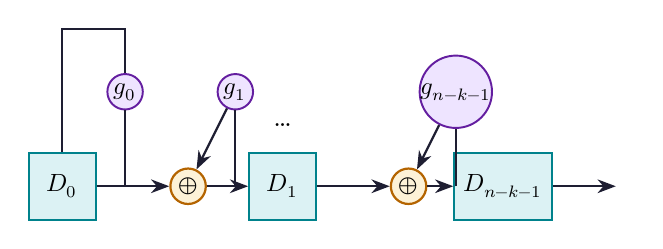
\begin{tikzpicture}[node distance=1.2cm]
  \node[reg] (r0) at (0,0) {$D_0$};
  \node[adder] (a1) at (1.6,0) {$\oplus$};
  \node[reg] (r1) at (2.8,0) {$D_1$};
  \node[adder] (a2) at (4.4,0) {$\oplus$};
  \node[reg] (r2) at (5.6,0) {$D_{n-k-1}$};

  \draw[arrow] (r0) -- (a1);
  \draw[arrow] (a1) -- (r1);
  \draw[arrow] (r1) -- (a2);
  \draw[arrow] (a2) -- (r2);

  \node[mult] (m0) at (0.8, 1.2) {$g_0$};
  \node[mult] (m1) at (2.2, 1.2) {$g_1$};
  \node[mult] (m2) at (5.0, 1.2) {$g_{n-k-1}$};

  \draw[line] (0.8, 0) -- (m0);
  \draw[line] (m0) |- (0, 2.0) -- (r0);
  
  \draw[line] (2.2, 0) -- (m1);
  \draw[arrow] (m1) -- (a1);

  \draw[line] (5.0, 0) -- (m2);
  \draw[arrow] (m2) -- (a2);
  
  \node[right=0.8cm of r2] (out) {};
  \draw[arrow] (r2) -- (out);
  
  \node[above=0.2cm of r1] {\dots};
\end{tikzpicture}
\end{tcolorbox}

The division operates as follows:
\begin{enumerate}[leftmargin=*, itemsep=3pt]
  \item The gate switch is closed. The $k$ message bits are fed into the channel and the feedback path simultaneously.
  \item After $k$ clock cycles, the shift registers contain the remainder coefficients (parity bits).
  \item The gate switch is opened, disabling feedback, and the parity bits are shifted out to complete the $n$-bit systematic codeword.
\end{enumerate}

\subsection{FSR Syndrome Calculator Circuit}
The syndrome $S(x)$ of a received polynomial $r(x)$ is the remainder of $r(x)$ divided by $g(x)$:
\[ S(x) = r(x) \pmod{g(x)} \]
This is implemented using a feedback shift register similar to the encoder.

\begin{tcolorbox}[tikzbox, title={Syndrome Calculator Circuit}]
\centering
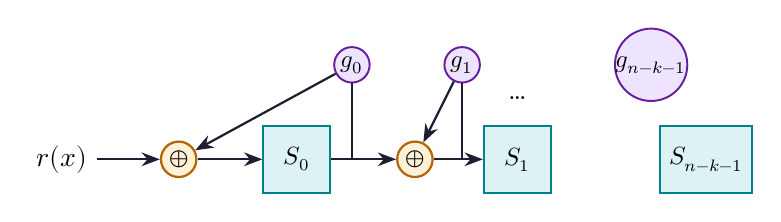
\begin{tikzpicture}[node distance=1.2cm]
  \node[adder] (inadd) at (-1.5, 0) {$\oplus$};
  \node[reg] (s0) at (0,0) {$S_0$};
  \node[adder] (sadd1) at (1.5,0) {$\oplus$};
  \node[reg] (s1) at (2.8,0) {$S_1$};
  \node[reg] (s2) at (5.2,0) {$S_{n-k-1}$};

  \draw[arrow] (inadd) -- (s0);
  \draw[arrow] (s0) -- (sadd1);
  \draw[arrow] (sadd1) -- (s1);
  
  \node[mult] (g0) at (0.7, 1.2) {$g_0$};
  \node[mult] (g1) at (2.1, 1.2) {$g_1$};
  \node[mult] (g2) at (4.5, 1.2) {$g_{n-k-1}$};

  \draw[line] (0.7, 0) -- (g0);
  \draw[arrow] (g0) -- (inadd);
  
  \draw[line] (2.1, 0) -- (g1);
  \draw[arrow] (g1) -- (sadd1);
  
  \node[left=0.8cm of inadd] (rx) {$r(x)$};
  \draw[arrow] (rx) -- (inadd);
  
  \node[above=0.2cm of s1] {\dots};
\end{tikzpicture}
\tcbset{after={\color{black}}}
\end{tcolorbox}

% ===============================================================================
\section{Spectral Properties of Cyclic Codes}
% ===============================================================================

Like time-domain signals, codewords of cyclic codes have equivalent frequency-domain descriptions using the \textbf{Discrete Fourier Transform (DFT)} over finite fields.
Let $v = (v_0, v_1, \dots, v_{n-1})$ be a vector over $\text{GF}(2^m)$ where $n$ divides $2^m - 1$. Let $\alpha$ be a primitive $n$-th root of unity in $\text{GF}(2^m)$.

\begin{tcolorbox}[defbox, title={\textbf{Finite Field Discrete Fourier Transform}}]
The DFT of $v$, denoted $V = (V_0, V_1, \dots, V_{n-1})$, consists of elements in $\text{GF}(2^m)$ computed by:
\[ V_j = \sum_{i=0}^{n-1} v_i \alpha^{ij}, \quad j = 0, 1, \dots, n-1 \]
The inverse DFT is:
\[ v_i = \sum_{j=0}^{n-1} V_j \alpha^{-ij}, \quad i = 0, 1, \dots, n-1 \]
\end{tcolorbox}

\subsection{Spectral Constraints and Ideals}
The cyclic shift of a vector $v$ in the time domain corresponds to multiplying its spectral components by powers of $\alpha$:
\[ v^{(1)} \longleftrightarrow (\alpha^0 V_0, \alpha^1 V_1, \dots, \alpha^{n-1} V_{n-1}) \]
Therefore, a cyclic code can be defined in the spectral domain by forcing certain spectral components to zero:
\[ C = \{ c \in \text{GF}(2)^n \mid C_j = 0 \text{ for all } j \in \mathcal{K} \} \]
where $\mathcal{K}$ is a set of spectral indices. This spectral property is the foundation for designing BCH and Reed-Solomon codes.

% ═══════════════════════════════════════════════════════════════════════════════
% QUICK REVISION PAGE
% ═══════════════════════════════════════════════════════════════════════════════
\newpage
\begin{center}
  {\large\bfseries\color{myred} Quick Revision --- Module 2}\\[3pt]
  {\small\color{mydark} Galois Fields \& Cyclic Codes $|$ PE-EC801C}
\end{center}
\noindent{\color{myred}\rule{\linewidth}{1.2pt}}
\vspace{4pt}

\begin{tcolorbox}[formulabox, title={\textbf{Key Formulas and Metrics at a Glance}}]
\renewcommand{\arraystretch}{1.35}
\begin{tabularx}{\linewidth}{B{5.0cm} X}
Galois Field order & $q = p^m$ ($p$ is prime characteristic) \\[4pt]
Roots of Unity factor & $X^n \oplus 1 = g(x) \cdot h(x)$ \\[4pt]
Generator degree & $\deg(g(x)) = n - k$ \\[4pt]
Systematic Codeword polynomial & $c(x) = x^{n-k}m(x) \oplus [x^{n-k}m(x) \pmod{g(x)}]$ \\[4pt]
Modulo-2 addition relation & $a(x) \oplus b(x) = a(x) - b(x)$ \\[4pt]
Parity relation & $g(x) \cdot h(x) \equiv 0 \pmod{X^n \oplus 1}$ \\[4pt]
Finite Field DFT spectrum & $V_j = \sum_{i=0}^{n-1} v_i \alpha^{ij}$ \\[4pt]
Conjugate elements of $\beta$ & $\beta^{2^0}, \beta^{2^1}, \beta^{2^2}, \dots, \beta^{2^{d-1}}$ \\[4pt]
Generator matrix polynomial & $G = \begin{bmatrix} g(x) \\ x g(x) \\ \vdots \\ x^{k-1}g(x) \end{bmatrix}$ in non-systematic form
\end{tabularx}
\end{tcolorbox}

\vspace{6pt}

\begin{tcolorbox}[defbox, title={\textbf{One-Line Definitions}}]
\begin{itemize}[leftmargin=*, itemsep=3pt, topsep=0pt]
  \item \textbf{Abelian Group:} A group where the binary operation is commutative ($a * b = b * a$).
  \item \textbf{Field:} An algebraic ring where multiplication is commutative and every non-zero element has a multiplicative inverse.
  \item \textbf{Galois Field:} A finite field containing a prime-power number of elements, denoted $\text{GF}(p^m)$.
  \item \textbf{Irreducible Polynomial:} A polynomial that cannot be factored into polynomials of lower degree over the same field.
  \item \textbf{Primitive Element:} An element whose powers generate all non-zero elements of a finite field.
  \item \textbf{Minimal Polynomial:} The lowest-degree binary polynomial having a field element (and its conjugates) as roots.
  \item \textbf{Cyclic Code:} A linear code where a cyclic shift of any codeword produces another valid codeword.
  \item \textbf{Generator Polynomial ($g(x)$):} The unique lowest-degree polynomial of a cyclic code, which divides $X^n \oplus 1$.
\end{itemize}
\end{tcolorbox}

\newpage

\begin{tcolorbox}[exambox, title={\textbf{Frequently Asked / Viva Questions}}]
\begin{enumerate}[topsep=0pt, label=\textbf{Q\arabic*.}, itemsep=5pt]
  \item \Q{What are the differences between groups, rings, and fields?}
    A group has one operation ($+$). A ring has two operations ($+$ and $\cdot$) and is an Abelian group under addition. A field is a commutative ring with a multiplicative identity where every non-zero element has a unique multiplicative inverse.
  \item \Q{Why do Galois Fields only exist for prime-power sizes $p^m$?}
    For fields of size $q$, the characteristic must be a prime $p$. The field forms a vector space over its prime subfield $\text{GF}(p)$ of dimension $m$. Therefore, the number of elements in the field is $p \times p \times \dots \times p = p^m$.
  \item \Q{How is systematic cyclic encoding performed algebraically?}
    First, the message $m(x)$ is multiplied by $x^{n-k}$ to shift it. Then, we find the remainder $d(x)$ of $x^{n-k}m(x)$ divided by $g(x)$. The systematic codeword polynomial is constructed as $c(x) = x^{n-k}m(x) \oplus d(x)$.
  \item \Q{Why must the generator polynomial $g(x)$ divide $X^n \oplus 1$?}
    A cyclic code of length $n$ is an ideal in the polynomial ring modulo $X^n \oplus 1$. The ideal is generated by $g(x)$. Since the identity codeword $0 \equiv X^n \oplus 1 \pmod{X^n \oplus 1}$ must be a multiple of $g(x)$, $g(x)$ must divide $X^n \oplus 1$.
  \item \Q{Explain how a feedback shift register circuit performs polynomial division.}
    FSRs use shift register stages as memory and XOR gates as modulo-2 adders. Feedback paths multiply register states by coefficients $g_i$. Feeding coefficients through the loop matches polynomial long division.
  \item \Q{What are conjugate elements in a finite field?}
    For an element $\beta \in \text{GF}(2^m)$, its conjugates over $\text{GF}(2)$ are its repeated squarings: $\{\beta, \beta^2, \beta^4, \dots, \beta^{2^{d-1}}\}$, where $d$ is the cycle length. They share the same minimal polynomial.
  \item \Q{What is the parity check polynomial $h(x)$ of a cyclic code?}
    The parity check polynomial is defined by $h(x) = (X^n \oplus 1) / g(x)$. It has degree $k$ and satisfies $c(x) \cdot h(x) \equiv 0 \pmod{X^n \oplus 1}$ for any codeword $c(x)$.
  \item \Q{What are the advantages of cyclic codes over general linear block codes?}
    Cyclic codes have rich algebraic properties allowing systematic design (like BCH codes). In hardware, encoding and syndrome calculations are implemented using simple feedback shift registers.
  \item \Q{What is a primitive polynomial?}
    A primitive polynomial of degree $m$ is an irreducible polynomial over $\text{GF}(2)$ that has a primitive element of $\text{GF}(2^m)$ as a root. Its roots generate the entire multiplicative group.
  \item \Q{Explain the spectral definition of cyclic codes.}
    Using the DFT over finite fields, cyclic shifts correspond to multiplying spectral elements by powers of $\alpha$. A cyclic code is defined by forcing specific spectral elements of the codewords to zero.
\end{enumerate}
\tcbset{after={\color{black}}}
\end{tcolorbox}

\vspace{6pt}

\begin{tcolorbox}[tikzbox, title={\textbf{Comparison of Linear Block Codes and Cyclic Codes}}]
\renewcommand{\arraystretch}{1.45}
\begin{tabularx}{\linewidth}{|B{3.2cm}|Y|Y|}
\hline
\textbf{Property} & \textbf{Linear Block Codes} & \textbf{Cyclic Codes} \\
\hline
Mathematical Model & Vector Spaces over $\text{GF}(2)$ & Ideals in the ring $\text{GF}(2)[x]/(X^n \oplus 1)$ \\
\hline
Defining Matrices & Generator $G$ and Parity $H$ & Generator $g(x)$ and Parity $h(x)$ polynomials \\
\hline
Encoding Hardware & Matrix multiplication circuits & Feedback Shift Registers (FSR) \\
\hline
Error Correction & Systematic bounding & Rich algebraic code design (BCH/RS) \\
\hline
\end{tabularx}
\end{tcolorbox}


% -- Module 3 -----------------------------------------------------------------
\modulestart{3}{BCH Codes --- Definition and Construction}

\section{BCH Codes --- Definition and Construction}
% ===============================================================================

Bose-Chaudhuri-Hocquenghem (\textbf{BCH}) codes are a powerful class of multiple-error-correcting cyclic codes. They allow for the precise design of codes that can correct a specific number of random errors $t$.

\subsection{Definition of Binary BCH Codes}
Let $\alpha$ be a primitive element of $\text{GF}(2^m)$, and let $n = 2^m-1$. A $t$-error correcting binary BCH code of length $n$ is defined as a cyclic code whose generator polynomial $g(x)$ has the following $2t$ consecutive powers of $\alpha$ as roots:
\[ \alpha^1, \alpha^2, \alpha^3, \dots, \alpha^{2t} \]
Therefore, the generator polynomial is the Least Common Multiple (\textbf{LCM}) of the minimal polynomials $m_i(x)$ of these roots:
\begin{tcolorbox}[formulabox, title={\textbf{BCH Generator Polynomial}}]
\[ g(x) = \text{lcm} \{ m_1(x), m_2(x), \dots, m_{2t}(x) \} \]
where $m_i(x)$ is the minimal polynomial of $\alpha^i$ over $\text{GF}(2)$.
\end{tcolorbox}

\subsection{Design Distance vs. Minimum Distance}
Because the generator polynomial has $2t$ consecutive powers of $\alpha$ as roots, the minimum distance $d_{min}$ of the BCH code satisfies the \textbf{BCH Bound}:
\[ d_{min} \ge 2t + 1 \]
The value $d_d = 2t + 1$ is called the \textbf{design distance} of the BCH code. In many cases, the actual minimum distance is exactly equal to the design distance, though it can sometimes exceed it.

\begin{tcolorbox}[examplebox, title={\textbf{Design of a 2-Error Correcting BCH Code of Length $n=15$}}]
We wish to design a $t=2$ error-correcting BCH code of length $n = 15 = 2^4 - 1 \implies m=4$.
The generator polynomial must have roots $\alpha^1, \alpha^2, \alpha^3, \alpha^4$.
We identify the minimal polynomials of these roots in $\text{GF}(16)$:
\begin{itemize}[leftmargin=*, itemsep=2pt]
  \item Root $\alpha^1, \alpha^2, \alpha^4$: conjugate class $\{\alpha, \alpha^2, \alpha^4, \alpha^8\}$ with minimal polynomial $m_1(x) = x^4 \oplus x \oplus 1$.
  \item Root $\alpha^3$: conjugate class $\{\alpha^3, \alpha^6, \alpha^{12}, \alpha^9\}$ with minimal polynomial $m_3(x) = x^4 \oplus x^3 \oplus x^2 \oplus x \oplus 1$.
\end{itemize}
Therefore, the generator polynomial is:
\[ g(x) = \text{lcm}\{m_1(x), m_3(x)\} = m_1(x) \cdot m_3(x) \]
\[ g(x) = (x^4 \oplus x \oplus 1)(x^4 \oplus x^3 \oplus x^2 \oplus x \oplus 1) = x^8 \oplus x^7 \oplus x^6 \oplus x^4 \oplus 1 \]
This is a $(15, 7)$ cyclic code. Since $\deg(g(x)) = 8$, the number of check bits is $8$, leaving $k = 7$ message bits. Its minimum distance satisfies $d_{min} \ge 2(2) + 1 = 5$.
\end{tcolorbox}

% ===============================================================================
\section{Idempotents and Mattson-Solomon Polynomials}
% ===============================================================================

\subsection{Idempotents}
In the algebra of cyclic codes (the ring $\text{GF}(2)[x] / (X^n \oplus 1)$), an \textbf{idempotent} is a polynomial $e(x)$ that is equal to its own square:
\[ e(x)^2 \equiv e(x) \pmod{X^n \oplus 1} \]
Every ideal (cyclic code) has a unique \textbf{generating idempotent} $e(x)$ which acts as the multiplicative identity of the code. The cyclic code can be defined directly by $e(x)$ rather than $g(x)$.

\subsection{Mattson-Solomon Polynomials}
The Mattson-Solomon polynomial represents a vector $v = (v_0, v_1, \dots, v_{n-1})$ of length $n$ (where $\gcd(n, p) = 1$) as a polynomial $g_v(z)$ over the extension field $\text{GF}(p^m)$:
\begin{tcolorbox}[defbox, title={\textbf{Mattson-Solomon Polynomial Definition}}]
\[ g_v(z) = \sum_{j=1}^n V_j z^{n-j} \]
where $V_j$ are the finite-field DFT coefficients of $v$:
\[ V_j = \sum_{i=0}^{n-1} v_i \alpha^{ij} \]
\end{tcolorbox}
The coefficients of $g_v(z)$ represent the spectral properties of the code, providing an elegant way to translate time-domain constraints into algebraic conditions.

% ===============================================================================
\section{Reed-Solomon Codes}
% ===============================================================================

\textbf{Reed-Solomon (RS)} codes are a non-binary subclass of BCH codes. Unlike binary codes, the elements of Reed-Solomon codewords are symbols from the Galois Field $\text{GF}(2^m)$ rather than individual bits.

\subsection{Basic Parameters}
Let $m$ be the number of bits per symbol.
\begin{tcolorbox}[defbox, title={\textbf{Reed-Solomon Parameters}}]
\begin{itemize}[leftmargin=*, itemsep=3pt, topsep=0pt]
  \item \textbf{Symbol size:} $m$ bits
  \item \textbf{Block length ($n$):} $n = 2^m - 1$ symbols (equivalent to $m(2^m-1)$ bits)
  \item \textbf{Message length ($k$):} $k$ symbols (equivalent to $m \cdot k$ bits)
  \item \textbf{Parity symbols ($n-k$):} $2t$ symbols
  \item \textbf{Minimum distance ($d_{min}$):} $d_{min} = n - k + 1$
\end{itemize}
\end{tcolorbox}

\begin{tcolorbox}[tikzbox, title={Reed-Solomon Codeword Structure}]
\centering
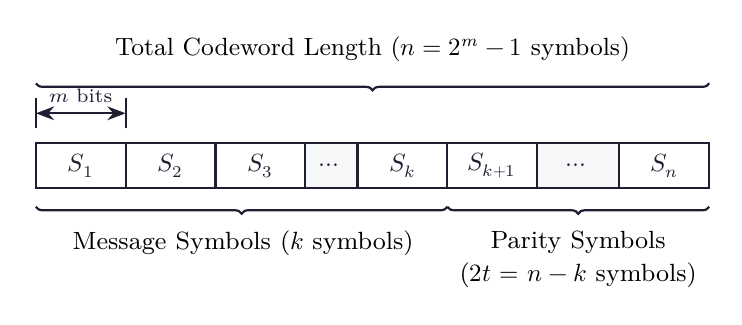
\begin{tikzpicture}[scale=0.95]
  % Draw individual cells
  \draw[line] (0,0.2) rectangle (1.2,0.8) node[pos=0.5, font=\small] {$S_1$};
  \draw[line] (1.2,0.2) rectangle (2.4,0.8) node[pos=0.5, font=\small] {$S_2$};
  \draw[line] (2.4,0.2) rectangle (3.6,0.8) node[pos=0.5, font=\small] {$S_3$};
  \draw[line, fill=mygray] (3.6,0.2) rectangle (4.3,0.8) node[pos=0.5, font=\small] {$\dots$};
  \draw[line] (4.3,0.2) rectangle (5.5,0.8) node[pos=0.5, font=\small] {$S_k$};
  \draw[line] (5.5,0.2) rectangle (6.7,0.8) node[pos=0.5, font=\small] {$S_{k+1}$};
  \draw[line, fill=mygray] (6.7,0.2) rectangle (7.8,0.8) node[pos=0.5, font=\small] {$\dots$};
  \draw[line] (7.8,0.2) rectangle (9,0.8) node[pos=0.5, font=\small] {$S_n$};
  
  % Braces for Message and Parity
  \draw[decoration={brace, mirror}, decorate, line, thick] (0, -0.05) -- (5.5, -0.05);
  \node[below=0.18cm, text width=5.2cm, align=center] at (2.75, -0.05) {\small Message Symbols ($k$ symbols)};
  
  \draw[decoration={brace, mirror}, decorate, line, thick] (5.5, -0.05) -- (9, -0.05);
  \node[below=0.18cm, text width=3.2cm, align=center] at (7.25, -0.05) {\small Parity Symbols ($2t = n-k$ symbols)};
  
  % Dimension indicator for one symbol (m bits)
  \draw[line] (0, 1.0) -- (0, 1.4);
  \draw[line] (1.2, 1.0) -- (1.2, 1.4);
  \draw[line, Stealth-Stealth] (0, 1.2) -- (1.2, 1.2) node[midway, above, font=\scriptsize] {$m$ bits};
  
  % Top brace for total length
  \draw[decoration={brace}, decorate, line, thick] (9, 1.6) -- (0, 1.6);
  \node[above=0.15cm] at (4.5, 1.6) {\small Total Codeword Length ($n = 2^m - 1$ symbols)};
\end{tikzpicture}
\end{tcolorbox}

\subsection{Error and Burst Correction Capability}
Since $d_{min} = n-k+1$, a Reed-Solomon code can correct up to $t$ symbol errors:
\[ t = \left\lfloor \frac{n-k}{2} \right\rfloor \]
RS codes are highly effective at correcting \textbf{burst errors} (consecutive bit errors). Since a symbol is treated as a single entity, if a burst of errors corrupts multiple bits within a single $m$-bit symbol, it counts as only \textbf{one symbol error}. A $t$-symbol correcting RS code can easily correct a continuous burst of errors up to $m(t-1) + 1$ bits.

% ===============================================================================
\section{MDS (Maximum Distance Separable) Codes}
% ===============================================================================

The Singleton bound states that for any linear block code with parameters $[n, k, d_{min}]$, the minimum distance is bounded by:
\[ d_{min} \le n - k + 1 \]

\begin{tcolorbox}[defbox, title={\textbf{MDS Code Definition}}]
A code is \textbf{Maximum Distance Separable (MDS)} if it meets the Singleton bound with strict equality:
\[ d_{min} = n - k + 1 \]
\end{tcolorbox}

\subsection{Properties of MDS Codes}
MDS codes are optimal because they achieve the maximum possible minimum distance for a given block length and code rate.
\begin{itemize}[leftmargin=*, itemsep=3pt]
  \item \textbf{Generator Matrix Independence:} A code is MDS if and only if \textbf{any $k$ columns} of its generator matrix $G$ are linearly independent.
  \item \textbf{Parity Matrix Independence:} A code is MDS if and only if \textbf{any $n-k$ columns} of its parity check matrix $H$ are linearly independent.
  \item \textbf{Dual Code:} The dual code of an MDS code is also an MDS code.
  \item \textbf{Examples:} Reed-Solomon codes are the most widely used class of MDS codes.
\end{itemize}

% ===============================================================================
\section{Justeen, Alterant and Goppa Codes}
% ===============================================================================

\subsection{Justeen Codes}
Justeen codes are a class of algebraic codes constructed by combining Reed-Solomon codes. They are designed to achieve good distance properties with simpler decoding algorithms.

\subsection{Alterant Codes}
Alterant codes are a generalization of BCH codes. They are defined by selecting roots from an extension field using a set of "locators" and "multipliers" that do not necessarily have the cyclic structure of standard BCH codes. This generalization allows for a wider choice of code lengths.

\subsection{Goppa Codes}
Goppa codes are an important class of non-cyclic algebraic codes defined by a \textbf{Goppa Polynomial} $g(z)$ over a finite field.
\begin{tcolorbox}[defbox, title={\textbf{Goppa Code Definition}}]
Let $L = \{\gamma_1, \gamma_2, \dots, \gamma_n\}$ be a set of distinct elements in $\text{GF}(2^m)$, and let $g(z)$ be a polynomial over $\text{GF}(2^m)$ such that $g(\gamma_i) \neq 0$ for all $i$. A Goppa code consists of all vectors $c = (c_1, \dots, c_n)$ that satisfy:
\[ \sum_{i=1}^n \frac{c_i}{z - \gamma_i} \equiv 0 \pmod{g(z)} \]
\end{tcolorbox}
Goppa codes are key to \textbf{code-based cryptography} (e.g., the McEliece cryptosystem) because their lack of cyclic structure makes them resistant to algebraic attacks while retaining strong error-correction capabilities.

\subsection{Generalized BCH Codes}
Generalized BCH codes extend standard BCH codes by relaxing the requirement that the roots be consecutive powers of a primitive element. By choosing an arbitrary set of roots, we can optimize the code for specific channels.

% ===============================================================================
\section{Code Classes Hierarchy}
% ===============================================================================

The relationship between the various algebraic code classes described can be represented as a hierarchical tree:

\begin{tcolorbox}[tikzbox, title={Algebraic Codes Hierarchy}]
\centering
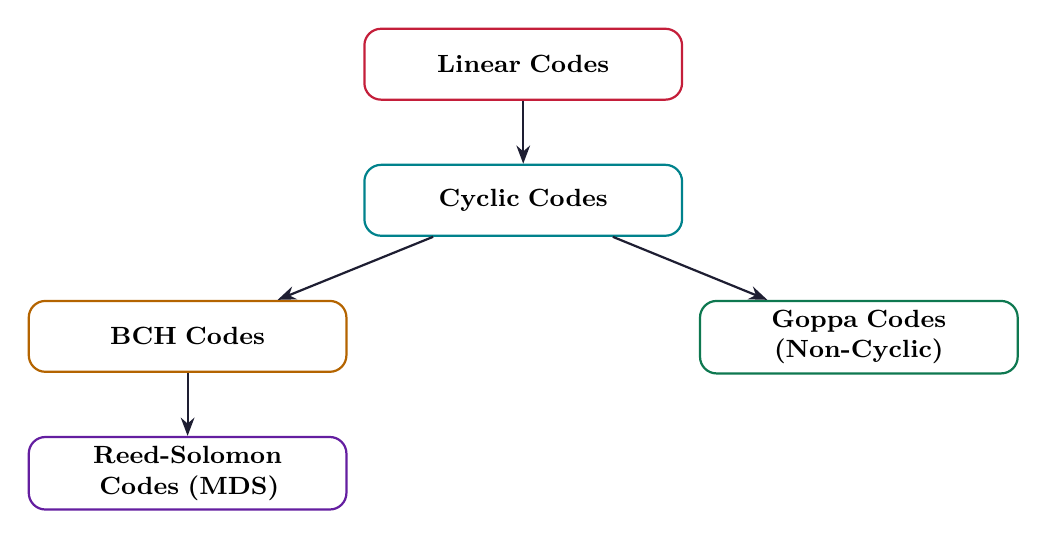
\begin{tikzpicture}[node distance=1.5cm and 0.5cm]
  \node[card, draw=myred] (lin) {Linear Codes};
  \node[card, draw=myteal, below=0.8cm of lin] (cyc) {Cyclic Codes};
  \node[card, draw=myamber, below left=0.8cm and 0.2cm of cyc] (bch) {BCH Codes};
  \node[card, draw=mygreen, below right=0.8cm and 0.2cm of cyc] (gop) {Goppa Codes (Non-Cyclic)};
  \node[card, draw=mypurple, below=0.8cm of bch] (rs) {Reed-Solomon Codes (MDS)};

  \draw[arrow] (lin) -- (cyc);
  \draw[arrow] (cyc) -- (bch);
  \draw[arrow] (cyc) -- (gop);
  \draw[arrow] (bch) -- (rs);
\end{tikzpicture}
\tcbset{after={\color{black}}}
\end{tcolorbox}

% ═══════════════════════════════════════════════════════════════════════════════
% QUICK REVISION PAGE
% ═══════════════════════════════════════════════════════════════════════════════
\newpage
\begin{center}
  {\large\bfseries\color{myred} Quick Revision --- Module 3}\\[3pt]
  {\small\color{mydark} BCH, RS and Special Codes $|$ PE-EC801C}
\end{center}
\noindent{\color{myred}\rule{\linewidth}{1.2pt}}
\vspace{4pt}

\begin{tcolorbox}[formulabox, title={\textbf{Key Formulas and Metrics at a Glance}}]
\renewcommand{\arraystretch}{1.35}
\begin{tabularx}{\linewidth}{B{5.0cm} X}
BCH roots criteria & $g(\alpha^i) = 0$ for $i = 1, 2, \dots, 2t$ \\[4pt]
BCH bound & $d_{min} \ge 2t + 1$ \\[4pt]
RS Block length (symbols) & $n = 2^m - 1$ \\[4pt]
RS Message length (symbols) & $k = n - 2t$ \\[4pt]
MDS Singleton equality & $d_{min} = n - k + 1$ \\[4pt]
RS Error correction capability & $t = \lfloor (n-k)/2 \rfloor$ symbol errors \\[4pt]
Idempotent condition & $e(x)^2 \equiv e(x) \pmod{X^n \oplus 1}$ \\[4pt]
Mattson-Solomon polynomial & $g_v(z) = \sum_{j=1}^n V_j z^{n-j}$ \\[4pt]
Goppa code congruence & $\sum_{i=1}^n \frac{c_i}{z - \gamma_i} \equiv 0 \pmod{g(z)}$
\end{tabularx}
\end{tcolorbox}

\vspace{6pt}

\begin{tcolorbox}[defbox, title={\textbf{One-Line Definitions}}]
\begin{itemize}[leftmargin=*, itemsep=3pt, topsep=0pt]
  \item \textbf{BCH Code:} A class of multiple-error-correcting cyclic codes defined by consecutive powers of $\alpha$ as roots.
  \item \textbf{Idempotent Polynomial:} A polynomial that is equal to its own square modulo $X^n \oplus 1$.
  \item \textbf{Reed-Solomon Code:} A non-binary subclass of BCH codes where symbols are from GF($2^m$).
  \item \textbf{Singleton Bound:} The upper limit on the minimum distance of a block code: $d_{min} \le n - k + 1$.
  \item \textbf{MDS Code:} A code that achieves the Singleton bound with equality.
  \item \textbf{Goppa Code:} A class of non-cyclic algebraic codes defined by a Goppa polynomial $g(z)$ over a finite field.
  \item \textbf{Burst Error:} A sequence of consecutive bit errors caused by channel disturbances.
  \item \textbf{Design Distance ($d_d$):} The lower bound on minimum distance ($2t+1$) used to construct a BCH code.
\end{itemize}
\end{tcolorbox}

\newpage

\begin{tcolorbox}[exambox, title={\textbf{Frequently Asked / Viva Questions}}]
\begin{enumerate}[topsep=0pt, label=\textbf{Q\arabic*.}, itemsep=5pt]
  \item \Q{How is a BCH generator polynomial constructed for a given error capability $t$?}
    We first identify the $2t$ consecutive roots: $\alpha^1, \dots, \alpha^{2t}$. Then, we find the minimal polynomials $m_i(x)$ for each of these roots. The generator polynomial is the least common multiple (LCM) of these minimal polynomials.
  \item \Q{Why are Reed-Solomon codes highly suited for burst error correction?}
    RS codes operate on $m$-bit symbols. An error burst of length $L$ bits can corrupt at most $\lceil L/m \rceil + 1$ symbols. Since correcting a symbol corrects all bit errors within it, RS codes handle localized burst corruptions very efficiently.
  \item \Q{What makes a code "Maximum Distance Separable" (MDS)?}
    A code is MDS if its minimum distance $d_{min}$ reaches the absolute theoretical maximum defined by the Singleton bound: $d_{min} = n - k + 1$. Reed-Solomon codes are the most famous example.
  \item \Q{Explain the role of the Goppa polynomial in cryptography.}
    Goppa codes are the foundation of McEliece cryptography. Because they lack cyclic structure, their generator matrices appear random to attackers, making it difficult to decode messages without the private Goppa polynomial.
  \item \Q{What is the difference between binary BCH codes and Reed-Solomon codes?}
    Binary BCH codes process individual bits, and their codewords consist of bits. RS codes are non-binary BCH codes where codewords consist of multi-bit symbols from GF($2^m$), offering better performance against symbol-level errors.
  \item \Q{What are idempotents and how do they relate to cyclic codes?}
    An idempotent is a polynomial satisfying $e(x)^2 \equiv e(x) \pmod{X^n \oplus 1}$. In cyclic codes, the generating idempotent serves as the identity element of the code and uniquely defines the ideal.
  \item \Q{Explain the Singleton bound and its implication.}
    The Singleton bound states $d_{min} \le n - k + 1$. It implies that the minimum distance cannot exceed the number of parity check bits plus one, representing the trade-off between redundancy and error capability.
  \item \Q{What are Justeen codes?}
    Justeen codes are algebraic codes built by combining Reed-Solomon codes, designed to achieve excellent distance properties with simpler, lower-complexity decoders.
  \item \Q{Define the Mattson-Solomon polynomial.}
    The Mattson-Solomon polynomial represents a vector as a polynomial $g_v(z) = \sum V_j z^{n-j}$ where $V_j$ are its finite field DFT coefficients, mapping time-domain data into the spectral domain.
  \item \Q{Is the actual minimum distance of a BCH code always equal to its design distance?}
    No. The BCH bound guarantees $d_{min} \ge 2t+1$. While the actual minimum distance is often equal to $2t+1$, it can sometimes be larger due to the properties of the minimal polynomials.
\end{enumerate}
\tcbset{after={\color{black}}}
\end{tcolorbox}

\vspace{6pt}

\begin{tcolorbox}[tikzbox, title={\textbf{Comparison of BCH and Reed-Solomon Codes}}]
\renewcommand{\arraystretch}{1.45}
\begin{tabularx}{\linewidth}{|B{3.2cm}|Y|Y|}
\hline
\textbf{Property} & \textbf{Binary BCH Codes} & \textbf{Reed-Solomon Codes} \\
\hline
Symbol Type & Binary bits ($0, 1$) & Non-binary symbols from $\text{GF}(2^m)$ \\
\hline
Block Length ($n$) & $2^m - 1$ bits & $2^m - 1$ symbols \\
\hline
Minimum Distance & $d_{min} \ge 2t + 1$ & $d_{min} = n - k + 1$ (MDS) \\
\hline
Error Target & Random single-bit errors & Burst errors and symbol-level corruptions \\
\hline
Complexity & Moderate & High (requires finite field arithmetic) \\
\hline
\end{tabularx}
\end{tcolorbox}


% -- Module 4 -----------------------------------------------------------------
\modulestart{4}{The BCH/RS Decoding Pipeline}

\section{The BCH/RS Decoding Pipeline}
% ===============================================================================

Decoding algebraic codes (BCH and Reed-Solomon) is more complex than decoding linear block codes. Instead of simple table lookups, a multi-stage algebraic pipeline computes error locations and error values.

\begin{tcolorbox}[tikzbox, title={BCH and Reed-Solomon Decoding Flowchart}]
\centering
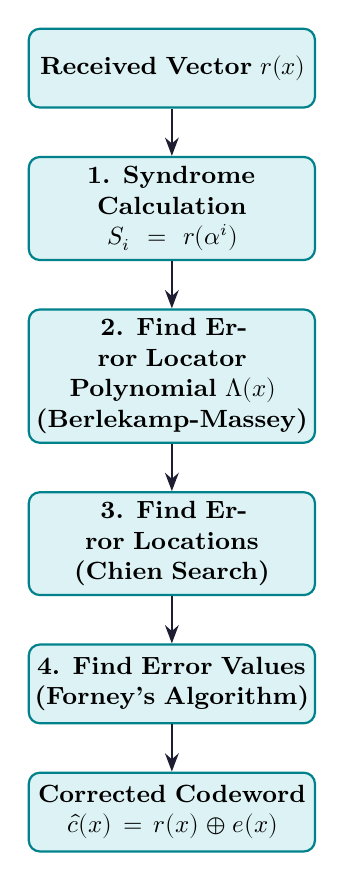
\begin{tikzpicture}[node distance=1.6cm]
  \node[stepnode] (n0) {Received Vector $r(x)$};
  \node[stepnode, below=0.6cm of n0] (n1) {1. Syndrome Calculation \\ $S_i = r(\alpha^i)$};
  \node[stepnode, below=0.6cm of n1] (n2) {2. Find Error Locator \\ Polynomial $\Lambda(x)$ \\ (Berlekamp-Massey)};
  \node[stepnode, below=0.6cm of n2] (n3) {3. Find Error Locations \\ (Chien Search)};
  \node[stepnode, below=0.6cm of n3] (n4) {4. Find Error Values \\ (Forney's Algorithm)};
  \node[stepnode, below=0.6cm of n4] (n5) {Corrected Codeword \\ $\hat{c}(x) = r(x) \oplus e(x)$};

  \draw[flowarrow] (n0) -- (n1);
  \draw[flowarrow] (n1) -- (n2);
  \draw[flowarrow] (n2) -- (n3);
  \draw[flowarrow] (n3) -- (n4);
  \draw[flowarrow] (n4) -- (n5);
\end{tikzpicture}
\end{tcolorbox}

% ===============================================================================
\section{Syndrome Polynomial and the Key Equation}
% ===============================================================================

Let $c(x)$ be the transmitted codeword polynomial, $r(x)$ be the received polynomial, and $e(x) = \sum_{j \in \mathcal{E}} Y_j x^j$ be the error polynomial, where $\mathcal{E}$ is the set of error positions and $Y_j$ are the error values ($Y_j \in \text{GF}(2)$ for binary BCH, and $Y_j \in \text{GF}(2^m)$ for RS codes).

\subsection{Syndrome Calculations}
The decoder calculates $2t$ syndromes:
\[ S_i = r(\alpha^i) = c(\alpha^i) \oplus e(\alpha^i) = 0 \oplus e(\alpha^i) = \sum_{l=1}^\nu Y_l X_l^i, \quad i = 1, 2, \dots, 2t \]
where $\nu$ is the actual number of errors, $X_l = \alpha^{i_l}$ is the \textbf{error locator} indicating the position of the $l$-th error, and $Y_l$ is the error value.
We define the \textbf{Syndrome Polynomial}:
\[ S(x) = \sum_{i=1}^{2t} S_i x^{i-1} = S_1 \oplus S_2 x \oplus S_3 x^2 \oplus \dots \oplus S_{2t} x^{2t-1} \]

\subsection{The Error Locator Polynomial}
The \textbf{Error Locator Polynomial} $\Lambda(x)$ has roots that are the reciprocals of the error locators $X_l$:
\begin{tcolorbox}[defbox, title={\textbf{Error Locator Polynomial}}]
\[ \Lambda(x) = \prod_{l=1}^\nu (1 - X_l x) = 1 + \Lambda_1 x + \Lambda_2 x^2 + \dots + \Lambda_\nu x^\nu \]
The roots of $\Lambda(x)$ are $x_l = X_l^{-1}$. Finding these roots reveals the error positions.
\end{tcolorbox}

\subsection{The Key Equation}
By defining the \textbf{Error Evaluator Polynomial} $\Omega(x)$ of degree less than $\nu$, we establish the fundamental relationship of algebraic decoding:
\begin{tcolorbox}[formulabox, title={\textbf{The Key Equation of Decoding}}]
\[ \Lambda(x) \cdot S(x) \equiv \Omega(x) \pmod{x^{2t}} \]
\end{tcolorbox}
The task of the decoder is to solve this equation for $\Lambda(x)$ and $\Omega(x)$, given the known syndrome polynomial $S(x)$.

% ===============================================================================
\section{The Berlekamp-Massey Algorithm}
% ===============================================================================

The \textbf{Berlekamp-Massey (BM)} algorithm is an iterative design procedure that solves the key equation. It views the syndrome values as outputs of a Linear Feedback Shift Register (LFSR) and finds the minimum register length $L$ and feedback connection polynomial $\Lambda^{(r)}(x)$ that can synthesize the sequence $S_1, S_2, \dots, S_{2t}$.

\subsection{Iterative Steps of the BM Algorithm}
We compute polynomials $\Lambda^{(r)}(x)$ for $r = 1, 2, \dots, 2t$:
\begin{tcolorbox}[formulabox, title={\textbf{Berlekamp-Massey Iteration}}]
At step $r$, we compute the \textbf{discrepancy} $d_r$:
\[ d_r = S_{r+1} \oplus \sum_{i=1}^L \Lambda_i^{(r)} S_{r+1-i} \]
\begin{enumerate}[leftmargin=*, itemsep=3pt, topsep=0pt]
  \item If $d_r = 0$, the current LFSR synthesizes the next syndrome:
    \[ \Lambda^{(r+1)}(x) = \Lambda^{(r)}(x), \quad L^{(r+1)} = L^{(r)} \]
  \item If $d_r \neq 0$, the loop coefficients must be adjusted:
    \[ \Lambda^{(r+1)}(x) = \Lambda^{(r)}(x) - d_r d_p^{-1} x^{r-p} \Lambda^{(p)}(x) \]
    where $p$ is a previous step that had a non-zero discrepancy $d_p$, chosen to minimize the new register length:
    \[ L^{(r+1)} = \max \left( L^{(r)}, \, r + 1 - L^{(r)} \right) \]
\end{enumerate}
\end{tcolorbox}
After $2t$ iterations, the resulting polynomial $\Lambda^{(2t)}(x)$ is the desired error locator polynomial $\Lambda(x)$.

% ===============================================================================
\section{Massey's Shift Register Synthesis}
% ===============================================================================

James Massey showed that the algebraic problem of decoding BCH codes is equivalent to the system-theoretic problem of synthesizing a minimum-length linear feedback shift register that generates a given sequence.

\begin{tcolorbox}[tikzbox, title={Massey's LFSR Synthesis Model}]
\centering
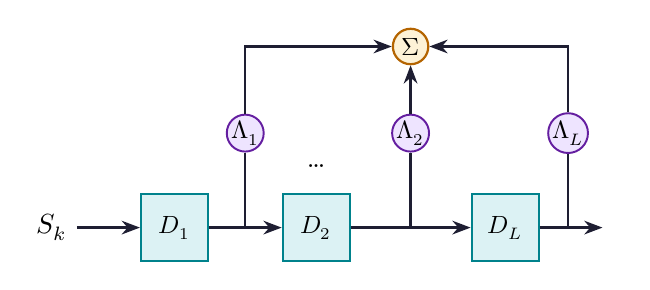
\begin{tikzpicture}[node distance=1.2cm]
  \node[reg] (s0) at (0,0) {$D_1$};
  \node[reg] (s1) at (1.8,0) {$D_2$};
  \node[reg] (s2) at (4.2,0) {$D_L$};

  \draw[arrow] (s0) -- (s1);
  \draw[arrow] (s1) -- (s2);

  \node[mult] (c1) at (0.9, 1.2) {$\Lambda_1$};
  \node[mult] (c2) at (3.0, 1.2) {$\Lambda_2$};
  \node[mult] (cL) at (5.0, 1.2) {$\Lambda_L$};

  \draw[line] (0.9, 0) -- (c1);
  \draw[line] (3.0, 0) -- (c2);
  \draw[line] (5.0, 0) -- (cL);

  \node[adder] (sum) at (3.0, 2.3) {$\Sigma$};
  \draw[arrow] (c1) |- (sum);
  \draw[arrow] (c2) -- (sum);
  \draw[arrow] (cL) |- (sum);

  \node[right=0.8cm of s2] (out) {};
  \draw[arrow] (s2) -- (out);

  \node[left=0.8cm of s0] (in) {$S_k$};
  \draw[arrow] (in) -- (s0);
  
  \node[above=0.2cm of s1] {\dots};
\end{tikzpicture}
\end{tcolorbox}

The feedback connections $\Lambda_1, \dots, \Lambda_L$ represent the coefficients of the error locator polynomial $\Lambda(x) = 1 + \Lambda_1 x + \dots + \Lambda_L x^L$. The discrepancy $d_r$ represents the difference between the actual syndrome $S_{r+1}$ and the output predicted by the shift register.

% ===============================================================================
\section{A Fast Berlekamp-Massey Algorithm}
% ===============================================================================

To handle high-speed data transmission (e.g., optical networks and solid-state storage), the iterative Berlekamp-Massey algorithm can be reorganized into a parallel, systolic architecture.
By utilizing division-free updates and maintaining auxiliary polynomials in parallel, modern decoders compute $\Lambda(x)$ in exactly $2t$ clock cycles without needing finite-field inversions ($d_p^{-1}$).

% ===============================================================================
\section{Chien Search and Forney's Algorithm}
% ===============================================================================

Once $\Lambda(x)$ and $\Omega(x)$ are computed, we must identify the error locations and calculate their values.

\subsection{Chien Search}
Chien search is a hardware-efficient method to find the roots of $\Lambda(x)$. Since the roots must lie in the finite field $\text{GF}(2^m)$, we test all possible elements $\alpha^{-i}$ ($i = 0, \dots, n-1$):
\[ \Lambda(\alpha^{-i}) = 1 + \Lambda_1 \alpha^{-i} + \Lambda_2 \alpha^{-2i} + \dots + \Lambda_\nu \alpha^{-\nu i} \]
If $\Lambda(\alpha^{-i}) = 0$, then position $i$ is identified as an error location.
In hardware, the terms $\Lambda_j \alpha^{-ji}$ are updated each clock cycle using simple scaling registers, avoiding expensive exponentiations.

\subsection{Forney's Algorithm}
For non-binary codes (like Reed-Solomon), we must find the error values $Y_l$ to correct the corrupted symbols. Forney's algorithm computes these directly:
\begin{tcolorbox}[formulabox, title={\textbf{Forney's Error Value Formula}}]
The error value $Y_l$ at position $i_l$ (where $X_l = \alpha^{i_l}$) is:
\[ Y_l = - \frac{\Omega(X_l^{-1})}{\Lambda'(X_l^{-1})} \]
where $\Lambda'(x)$ is the formal derivative of the error locator polynomial:
\[ \Lambda'(x) = \sum_{j=1}^\nu j \cdot \Lambda_j x^{j-1} \]
\end{tcolorbox}
In binary fields, the addition is modulo-2, so the negative sign is ignored, and the derivative $\Lambda'(x)$ simplifies to the sum of its odd-indexed terms.

% ═══════════════════════════════════════════════════════════════════════════════
% QUICK REVISION PAGE
% ═══════════════════════════════════════════════════════════════════════════════
\newpage
\begin{center}
  {\large\bfseries\color{myred} Quick Revision --- Module 4}\\[3pt]
  {\small\color{mydark} Decoding of BCH and RS Codes $|$ PE-EC801C}
\end{center}
\noindent{\color{myred}\rule{\linewidth}{1.2pt}}
\vspace{4pt}

\begin{tcolorbox}[formulabox, title={\textbf{Key Formulas and Metrics at a Glance}}]
\renewcommand{\arraystretch}{1.35}
\begin{tabularx}{\linewidth}{B{5.0cm} X}
Syndrome elements & $S_i = \sum_{l=1}^\nu Y_l X_l^i$ \\[4pt]
Syndrome Polynomial & $S(x) = \sum_{i=1}^{2t} S_i x^{i-1}$ \\[4pt]
Error Locator Polynomial & $\Lambda(x) = \prod_{l=1}^\nu (1 - X_l x)$ \\[4pt]
Key Equation of Decoding & $\Lambda(x) \cdot S(x) \equiv \Omega(x) \pmod{x^{2t}}$ \\[4pt]
Discrepancy equation & $d_r = S_{r+1} \oplus \sum_{i=1}^L \Lambda_i^{(r)} S_{r+1-i}$ \\[4pt]
Register length update & $L^{(r+1)} = \max \left( L^{(r)}, \, r + 1 - L^{(r)} \right)$ \\[4pt]
Chien search check & $\Lambda(\alpha^{-i}) = 0 \implies$ error at index $i$ \\[4pt]
Forney's error value & $Y_l = - \frac{\Omega(X_l^{-1})}{\Lambda'(X_l^{-1})}$ \\[4pt]
Formal derivative (binary) & $\Lambda'(x) = \Lambda_1 \oplus \Lambda_3 x^2 \oplus \Lambda_5 x^4 \oplus \dots$
\end{tabularx}
\end{tcolorbox}

\vspace{6pt}

\begin{tcolorbox}[defbox, title={\textbf{One-Line Definitions}}]
\begin{itemize}[leftmargin=*, itemsep=3pt, topsep=0pt]
  \item \textbf{Syndrome Polynomial ($S(x)$):} A polynomial constructed from received syndromes representing the error pattern.
  \item \textbf{Error Locator ($\Lambda(x)$):} A polynomial whose roots indicate the positions where transmission errors occurred.
  \item \textbf{Error Evaluator ($\Omega(x)$):} A polynomial containing spectral details used to calculate error magnitudes.
  \item \textbf{Discrepancy ($d_r$):} The difference between the observed syndrome and the LFSR prediction in BM.
  \item \textbf{Berlekamp-Massey Algorithm:} An iterative, FSR-based procedure used to solve the key equation.
  \item \textbf{Chien Search:} A systematic search method evaluating $\Lambda(x)$ at all field elements to find roots.
  \item \textbf{Forney's Algorithm:} A low-complexity algebraic method used to calculate error values for non-binary codes.
  \item \textbf{Key Equation:} The core modular relationship linking $\Lambda(x)$, $S(x)$, and $\Omega(x)$ in algebraic decoding.
\end{itemize}
\end{tcolorbox}

\newpage

\begin{tcolorbox}[exambox, title={\textbf{Frequently Asked / Viva Questions}}]
\begin{enumerate}[topsep=0pt, label=\textbf{Q\arabic*.}, itemsep=5pt]
  \item \Q{What are the four main steps of the BCH/RS decoding pipeline?}
    First, compute the syndrome values from the received vector. Second, apply the Berlekamp-Massey algorithm to compute the error locator polynomial $\Lambda(x)$. Third, perform Chien search to find the roots of $\Lambda(x)$, locating the errors. Fourth, use Forney's algorithm to compute error values.
  \item \Q{State the Key Equation of decoding and define its terms.}
    The Key Equation is $\Lambda(x) \cdot S(x) \equiv \Omega(x) \pmod{x^{2t}}$, where $\Lambda(x)$ is the error locator polynomial, $S(x)$ is the syndrome polynomial, and $\Omega(x)$ is the error evaluator polynomial. It links the time and spectral representations of errors.
  \item \Q{How does the Berlekamp-Massey algorithm model the decoding problem?}
    The BM algorithm models the syndrome sequence as outputs of a Linear Feedback Shift Register (LFSR). It iteratively constructs the shortest LFSR that generates the syndromes, which represents the minimum-degree error locator.
  \item \Q{Explain the concept of 'discrepancy' in the BM algorithm.}
    Discrepancy ($d_r$) is the difference between the actual syndrome $S_{r+1}$ and the value predicted by the feedback connections of the current iteration. If $d_r = 0$, the connections are correct; if $d_r \neq 0$, the connection polynomial must be adjusted.
  \item \Q{What is Chien search, and how does it optimize hardware implementation?}
    Chien search finds the roots of $\Lambda(x)$ by evaluating it at all field elements $\alpha^{-i}$. In hardware, terms are updated using multipliers that scale by constant values (powers of $\alpha$), replacing complex exponentiations with simple shifts.
  \item \Q{Explain Forney's algorithm and why it is useful.}
    Forney's algorithm calculates error values using $Y_l = -\Omega(X_l^{-1})/\Lambda'(X_l^{-1})$. It is highly useful because it allows direct computation of error values at known error locations without solving a large system of simultaneous equations.
  \item \Q{Why does the formal derivative of a polynomial simplify in binary fields?}
    In binary fields, addition is modulo-2. Since $2 \equiv 0 \pmod 2$, all terms with even powers in the derivative disappear (since their derivatives contain an even multiplier: $2 \cdot c \cdot x = 0$). Thus, only the odd-indexed terms remain.
  \item \Q{Can the BM algorithm handle erasure decoding?}
    Yes. Erasures are errors with known locations but unknown values. The BM algorithm can be initialized with an erasure locator polynomial, reducing the number of syndrome iterations needed to solve for the remaining unknown errors.
  \item \Q{What is the difference between Berlekamp-Massey and the Euclidean decoding algorithm?}
    BM is an iterative LFSR design process that runs in $2t$ steps. The Euclidean algorithm solves the key equation by finding the greatest common divisor of $x^{2t}$ and $S(x)$ using polynomial division. Both produce identical results.
  \item \Q{What happens during decoding if the number of channel errors exceeds $t$?}
    If the number of errors exceeds $t$, the Berlekamp-Massey algorithm will still compute a polynomial, but it will have invalid roots, or the roots won't correspond to correct locations, resulting in a decoding failure or undetected error.
\end{enumerate}
\tcbset{after={\color{black}}}
\end{tcolorbox}

\vspace{6pt}

\begin{tcolorbox}[tikzbox, title={\textbf{Comparison of Decoding Algorithms}}]
\renewcommand{\arraystretch}{1.45}
\begin{tabularx}{\linewidth}{|B{3.2cm}|Y|Y|}
\hline
\textbf{Property} & \textbf{Berlekamp-Massey Algorithm} & \textbf{Euclidean Algorithm} \\
\hline
Mathematical Basis & Linear feedback shift register synthesis & Polynomial GCD division \\
\hline
Execution Flow & Iterative (updates loop coefficients) & Recursive division steps \\
\hline
Hardware Suitability & Excellent (systolic array architectures) & Challenging (requires polynomial dividers) \\
\hline
Design Focus & Solving the LFSR feedback connections & Direct fraction reduction of $S(x)/x^{2t}$ \\
\hline
\end{tabularx}
\end{tcolorbox}


% -- Module 5 -----------------------------------------------------------------
\modulestart{5}{Introduction to Convolutional Codes}

\section{Introduction to Convolutional Codes}
% ===============================================================================

Unlike linear block codes, which segment the incoming message sequence into independent blocks of length $k$, \textbf{convolutional codes} process the message continuously. The coded output depends not only on the current input block but also on a finite number of previous input blocks stored in memory.

\subsection{Core Parameters}
A convolutional encoder is characterized by three main parameters:
\begin{enumerate}[leftmargin=*, itemsep=3pt]
  \item \textbf{Code Rate (\texorpdfstring{$R$}{R}):} Defined as $R = k/n$, where $k$ input bits produce $n$ output bits in each encoding cycle.
  \item \textbf{Memory Stages (\texorpdfstring{$M$}{M}):} The number of delay elements (flip-flops) in the shift registers.
  \item \textbf{Constraint Length (\texorpdfstring{$K$}{K}):} There are two standard definitions:
    \begin{itemize}[leftmargin=*, itemsep=2pt]
      \item \textbf{System-Theoretic definition:} $K = M + 1$. This represents the maximum number of input cycles over which a single input bit can influence the encoder's output.
      \item \textbf{Alternative definition:} $K = L \cdot k$, where $L$ is the number of stages in the shift register.
    \end{itemize}
\end{enumerate}

\subsection{Mathematical Representations}
The encoding operation can be described in three algebraic formats:
\begin{tcolorbox}[defbox, title={\textbf{Mathematical Formulations of Convolutional Coding}}]
\begin{enumerate}[leftmargin=*, itemsep=3pt, topsep=0pt]
  \item \textbf{Impulse Response:} Let $h^{(j)} = (h^{(j)}_0, h^{(j)}_1, \dots)$ be the impulse response of the path from the input to output $j$. For input sequence $u = (u_0, u_1, \dots)$, the output $v^{(j)}$ is the discrete convolution:
    \[ v^{(j)}_t = \sum_{i=0}^M u_{t-i} h^{(j)}_i \]
  \item \textbf{Generator Matrix (\texorpdfstring{$G$}{G}):} A semi-infinite, Block-Toeplitz matrix of the form:
    \[ G = \begin{bmatrix} 
      G_0 & G_1 & G_2 & \dots & G_M & 0 & \dots \\
      0   & G_0 & G_1 & \dots & G_{M-1} & G_M & \dots \\
      0   & 0   & G_0 & \dots & G_{M-2} & G_{M-1} & \dots \\
      \vdots & \vdots & \vdots & \ddots & \vdots & \vdots & \ddots
    \end{bmatrix} \]
    where each $G_i$ is a $k \times n$ sub-matrix representing tap connections.
  \item \textbf{Generator Polynomials:} Tap connections for the $j$-th output are expressed as a polynomial in the delay operator $D$:
    \[ g^{(j)}(D) = g^{(j)}_0 \oplus g^{(j)}_1 D \oplus g^{(j)}_2 D^2 \oplus \dots \oplus g^{(j)}_M D^M \]
\end{enumerate}
\end{tcolorbox}

% ===============================================================================
\section{Structural Representations}
% ===============================================================================

Convolutional encoders are implemented using feed-forward shift registers and modulo-2 adders. They can be analyzed using three graphical models.

\begin{tcolorbox}[tikzbox, title={Feed-Forward Encoder for a Rate 1/2 (\texorpdfstring{$K=3$}{K=3}) Convolutional Code}]
\centering
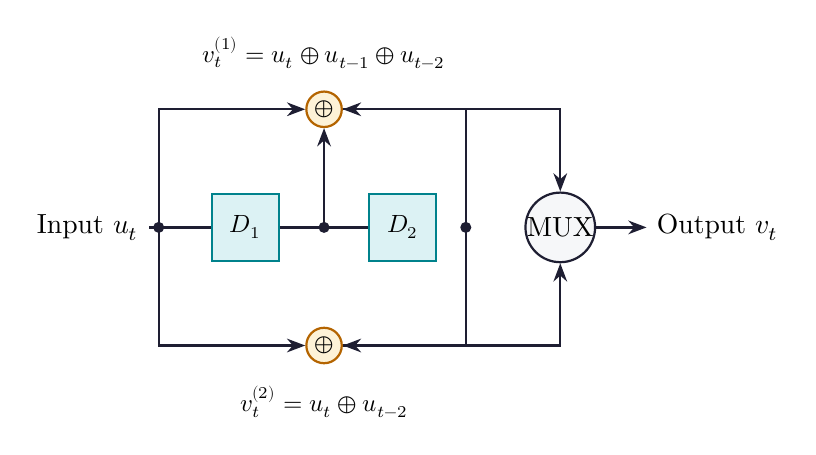
\begin{tikzpicture}[node distance=1.5cm, >=Stealth, thick]
  % Nodes
  \node (in) at (0,0) {Input $u_t$};
  \node[reg] (d1) at (2.0, 0) {$D_1$};
  \node[reg] (d2) at (4.0, 0) {$D_2$};
  
  % Modulo-2 adders
  \node[adder] (add1) at (3.0, 1.5) {$\oplus$};
  \node[adder] (add2) at (3.0, -1.5) {$\oplus$};
 
  % Output nodes
  \node[circle, draw=mydark, fill=mygray, minimum size=0.7cm, inner sep=0pt] (mux) at (6.0, 0) {MUX};
  \node (out) at (8.0, 0) {Output $v_t$};
 
  % Connections along main line
  \draw[line] (in) -- (d1);
  \draw[line] (d1) -- (d2);
 
  % Taps (coordinates along the line)
  \coordinate (tap0) at (0.9, 0);
  \coordinate (tap1) at (3.0, 0);
  \coordinate (tap2) at (4.8, 0);
 
  % Draw connection dots
  \fill[mydark] (tap0) circle (2pt);
  \fill[mydark] (tap1) circle (2pt);
  \fill[mydark] (tap2) circle (2pt);
 
  % Tap lines to Adder 1
  \draw[arrow] (tap0) |- (add1);
  \draw[arrow] (tap1) -- (add1);
  \draw[arrow] (tap2) |- (add1);
 
  % Tap lines to Adder 2
  \draw[arrow] (tap0) |- (add2);
  \draw[arrow] (tap2) |- (add2);
 
  % Adder to MUX
  \draw[arrow] (add1) -| (mux);
  \draw[arrow] (add2) -| (mux);
  \draw[arrow] (mux) -- (out);
 
  % Labels for outputs
  \node[above=0.15cm of add1] {\small $v^{(1)}_t = u_t \oplus u_{t-1} \oplus u_{t-2}$};
  \node[below=0.15cm of add2] {\small $v^{(2)}_t = u_t \oplus u_{t-2}$};
\end{tikzpicture}
\end{tcolorbox}

\subsection{State Transition Diagram}
A state transition diagram represents the encoder as a finite-state machine. The state is determined by the previous bits stored in the shift register: $S_t = (u_{t-1}, u_{t-2}, \dots, u_{t-M})$. For $M=2$, there are four possible states: $00$, $10$, $01$, and $11$.

\begin{tcolorbox}[tikzbox, title={State Transition Diagram (4-State, K=3 Encoder)}]
\centering
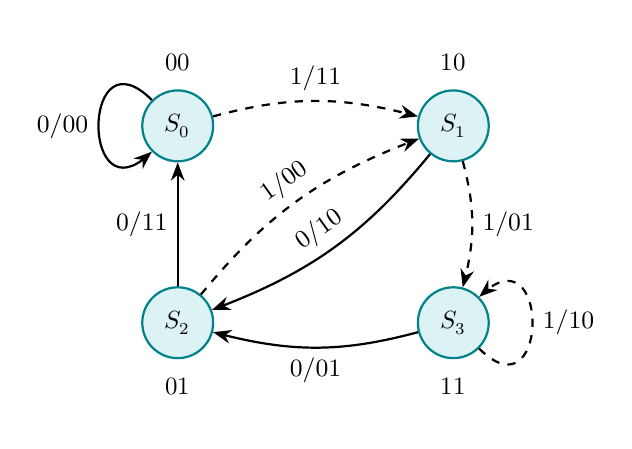
\begin{tikzpicture}[node distance=2.2cm, >=Stealth, thick]
  % Define states
  \node[state] (s0) at (0, 2) {$S_0$};
  \node[state] (s1) at (3.5, 2) {$S_1$};
  \node[state] (s2) at (0, -0.5) {$S_2$};
  \node[state] (s3) at (3.5, -0.5) {$S_3$};

  % Labels for states
  \node[above=0.1cm of s0] {\small $00$};
  \node[above=0.1cm of s1] {\small $10$};
  \node[below=0.1cm of s2] {\small $01$};
  \node[below=0.1cm of s3] {\small $11$};

  % Transitions
  % S0 loop
  \draw[->] (s0) to[out=135, in=225, looseness=5] node[left]{\small 0/00} (s0);
  % S0 to S1
  \draw[->, dashed] (s0) to[bend left=15] node[above]{\small 1/11} (s1);
  % S1 to S2
  \draw[->] (s1) to[bend left=15] node[above, sloped]{\small 0/10} (s2);
  % S1 to S3
  \draw[->, dashed] (s1) to[bend left=15] node[right]{\small 1/01} (s3);
  % S2 to S0
  \draw[->] (s2) to node[left]{\small 0/11} (s0);
  % S2 to S1
  \draw[->, dashed] (s2) to[bend left=15] node[above, sloped]{\small 1/00} (s1);
  % S3 to S2
  \draw[->] (s3) to[bend left=15] node[below]{\small 0/01} (s2);
  % S3 loop
  \draw[->, dashed] (s3) to[out=315, in=45, looseness=5] node[right]{\small 1/10} (s3);
\end{tikzpicture}
\par\vspace{3pt}\noindent
\small\textbf{Legend:} Solid lines represent transitions caused by input `0'. Dashed lines represent transitions caused by input `1'. Labels indicate \texttt{Input/Output}.
\end{tcolorbox}

\subsection{Tree Diagram}
The tree diagram represents all possible output paths starting from the initial state $00$. For each incoming bit, the path splits into two branches: the upper branch represents input $0$, and the lower branch represents input $1$. The diagram grows exponentially, making it suitable only for illustrating short sequences.

\begin{tcolorbox}[tikzbox, title={3-Level Tree Diagram Representation}]
\centering
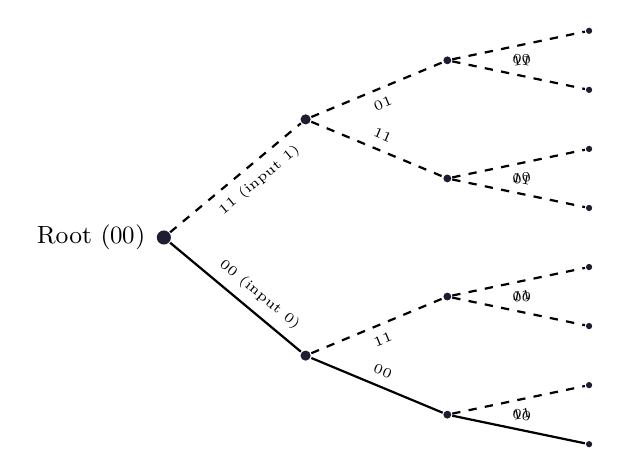
\begin{tikzpicture}[level distance=1.8cm,
  level 1/.style={sibling distance=3.0cm},
  level 2/.style={sibling distance=1.5cm},
  level 3/.style={sibling distance=0.75cm},
  grow=right, >=Stealth, thick]
  
  \node[circle, fill=mydark, inner sep=1.8pt, label=left:{\small Root ($00$)}] (root) {}
    child {
      node[circle, fill=mydark, inner sep=1.3pt] {}
      child {
        node[circle, fill=mydark, inner sep=1.0pt] {}
        child {
          node[circle, fill=mydark, inner sep=0.8pt] {}
          edge from parent node[above, sloped, pos=0.5] {\tiny 00}
        }
        child[dashed] {
          node[circle, fill=mydark, inner sep=0.8pt] {}
          edge from parent node[below, sloped, pos=0.5] {\tiny 11}
        }
        edge from parent node[above, sloped, pos=0.5] {\tiny 00}
      }
      child[dashed] {
        node[circle, fill=mydark, inner sep=1.0pt] {}
        child {
          node[circle, fill=mydark, inner sep=0.8pt] {}
          edge from parent node[above, sloped, pos=0.5] {\tiny 10}
        }
        child[dashed] {
          node[circle, fill=mydark, inner sep=0.8pt] {}
          edge from parent node[below, sloped, pos=0.5] {\tiny 01}
        }
        edge from parent node[below, sloped, pos=0.5] {\tiny 11}
      }
      edge from parent node[above, sloped, pos=0.6] {\tiny 00 (input 0)}
    }
    child[dashed] {
      node[circle, fill=mydark, inner sep=1.3pt] {}
      child {
        node[circle, fill=mydark, inner sep=1.0pt] {}
        child {
          node[circle, fill=mydark, inner sep=0.8pt] {}
          edge from parent node[above, sloped, pos=0.5] {\tiny 11}
        }
        child[dashed] {
          node[circle, fill=mydark, inner sep=0.8pt] {}
          edge from parent node[below, sloped, pos=0.5] {\tiny 00}
        }
        edge from parent node[above, sloped, pos=0.5] {\tiny 11}
      }
      child[dashed] {
        node[circle, fill=mydark, inner sep=1.0pt] {}
        child {
          node[circle, fill=mydark, inner sep=0.8pt] {}
          edge from parent node[above, sloped, pos=0.5] {\tiny 01}
        }
        child[dashed] {
          node[circle, fill=mydark, inner sep=0.8pt] {}
          edge from parent node[below, sloped, pos=0.5] {\tiny 10}
        }
        edge from parent node[below, sloped, pos=0.5] {\tiny 01}
      }
      edge from parent node[below, sloped, pos=0.6] {\tiny 11 (input 1)}
    };
\end{tikzpicture}
\end{tcolorbox}

\subsection{Trellis Diagram}
By merging node branches corresponding to identical states in the tree diagram, we obtain the \textbf{trellis diagram}. The trellis diagram is a time-indexed state diagram. Since the number of states is fixed ($2^M$), the trellis width is constant for all time intervals $t \ge M$, providing a highly compact layout for analyzing long sequences.

\begin{tcolorbox}[tikzbox, title={Trellis Diagram Section showing State Transitions and Survivor Path}]
\centering
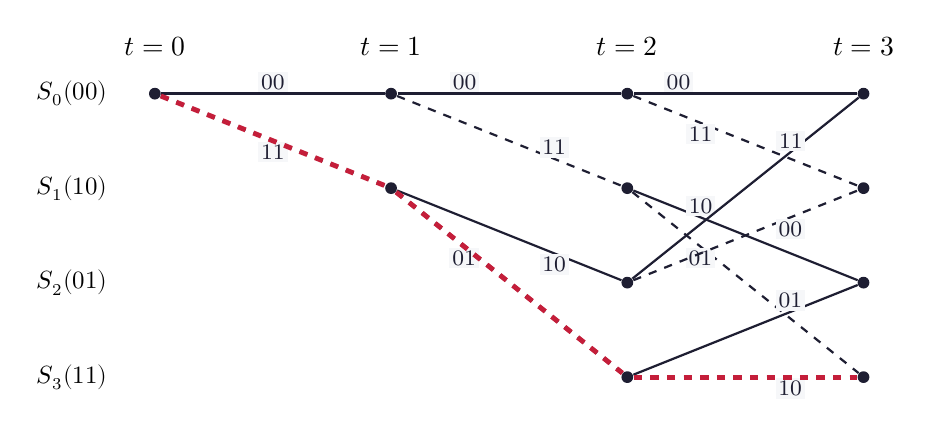
\begin{tikzpicture}[node distance=1.5cm, scale=1.2]
  % Define time steps
  \foreach \t in {0,1,2,3} {
    \node at (\t*2.5, 3.5) {\textbf{$t = \t$}};
  }
  
  % State vertical axis labels on the left
  \node[left] at (-0.4, 3) {\small $S_0(00)$};
  \node[left] at (-0.4, 2) {\small $S_1(10)$};
  \node[left] at (-0.4, 1) {\small $S_2(01)$};
  \node[left] at (-0.4, 0) {\small $S_3(11)$};

  % Draw states for each time step
  % t=0
  \node[trellisnode] (s0_0) at (0,3) {};
  
  % t=1
  \node[trellisnode] (s0_1) at (2.5,3) {};
  \node[trellisnode] (s1_1) at (2.5,2) {};
  
  % t=2
  \node[trellisnode] (s0_2) at (5,3) {};
  \node[trellisnode] (s1_2) at (5,2) {};
  \node[trellisnode] (s2_2) at (5,1) {};
  \node[trellisnode] (s3_2) at (5,0) {};
  
  % t=3
  \node[trellisnode] (s0_3) at (7.5,3) {};
  \node[trellisnode] (s1_3) at (7.5,2) {};
  \node[trellisnode] (s2_3) at (7.5,1) {};
  \node[trellisnode] (s3_3) at (7.5,0) {};

  % Draw transitions
  % t=0 to t=1
  \draw[line] (s0_0) -- node[above, pos=0.5, fill=mygray, inner sep=1pt]{\footnotesize 00} (s0_1);
  \draw[line, dashed] (s0_0) -- node[below, pos=0.5, fill=mygray, inner sep=1pt]{\footnotesize 11} (s1_1);
  
  % t=1 to t=2
  \draw[line] (s0_1) -- node[above, pos=0.3, fill=mygray, inner sep=1pt]{\footnotesize 00} (s0_2);
  \draw[line, dashed] (s0_1) -- node[above, pos=0.7, fill=mygray, inner sep=1pt]{\footnotesize 11} (s1_2);
  \draw[line] (s1_1) -- node[below, pos=0.7, fill=mygray, inner sep=1pt]{\footnotesize 10} (s2_2);
  \draw[line, dashed] (s1_1) -- node[below, pos=0.3, fill=mygray, inner sep=1pt]{\footnotesize 01} (s3_2);
  
  % t=2 to t=3
  \draw[line] (s0_2) -- node[above, pos=0.2, fill=mygray, inner sep=1pt]{\footnotesize 00} (s0_3);
  \draw[line, dashed] (s0_2) -- node[below, pos=0.3, fill=mygray, inner sep=1pt]{\footnotesize 11} (s1_3);
  
  \draw[line] (s1_2) -- node[above, pos=0.3, fill=mygray, inner sep=1pt]{\footnotesize 10} (s2_3);
  \draw[line, dashed] (s1_2) -- node[below, pos=0.3, fill=mygray, inner sep=1pt]{\footnotesize 01} (s3_3);
  
  \draw[line] (s2_2) -- node[above, pos=0.7, fill=mygray, inner sep=1pt]{\footnotesize 11} (s0_3);
  \draw[line, dashed] (s2_2) -- node[below, pos=0.7, fill=mygray, inner sep=1pt]{\footnotesize 00} (s1_3);
  
  \draw[line] (s3_2) -- node[above, pos=0.7, fill=mygray, inner sep=1pt]{\footnotesize 01} (s2_3);
  \draw[line, dashed] (s3_2) -- node[below, pos=0.7, fill=mygray, inner sep=1pt]{\footnotesize 10} (s3_3);

  % Highlight survivor path: s0_0 -> s1_1 -> s3_2 -> s3_3
  \draw[line, color=myred, line width=1.8pt, dashed] (s0_0) -- (s1_1);
  \draw[line, color=myred, line width=1.8pt, dashed] (s1_1) -- (s3_2);
  \draw[line, color=myred, line width=1.8pt, dashed] (s3_2) -- (s3_3);
\end{tikzpicture}
\end{tcolorbox}

% ===============================================================================
\section{Distance Properties of Convolutional Codes}
% ===============================================================================

The error-correcting capability of a convolutional code depends on its distance properties.

\subsection{Free Distance (\texorpdfstring{$d_{\text{free}}$}{dfree})}
The most important distance metric is the \textbf{free distance} $d_{\text{free}}$.
\begin{tcolorbox}[defbox, title={\textbf{Free Distance Definition}}]
The free distance $d_{\text{free}}$ is the minimum Hamming distance between any two distinct code sequences in the trellis that begin at state $00$ and eventually diverge, only to merge back at state $00$ at some later step.
\[ d_{\text{free}} = \min \left\{ d_H(v^{(1)}, v^{(2)}) \mid u^{(1)} \neq u^{(2)} \right\} \]
\end{tcolorbox}
If we set one sequence to be the all-zero codeword, $d_{\text{free}}$ simplifies to the minimum weight of a non-zero code sequence starting and ending at state $00$.
The number of errors $t$ that the code can correct is:
\[ t = \left\lfloor \frac{d_{\text{free}} - 1}{2} \right\rfloor \]

\subsection{Catastrophic Error Propagation}
Catastrophic error propagation is a key hazard in convolutional code design.
\begin{tcolorbox}[defbox, title={\textbf{Catastrophic Error Propagation}}]
A code is \textbf{catastrophic} if a finite number of channel transmission errors leads to an infinite number of decoding decisions/bit errors in the reconstructed message sequence.
\end{tcolorbox}
\textbf{Sufficient Condition:} In the state transition diagram of a catastrophic code, there exists a closed loop (cycle) containing a state other than $00$ where all transitions along the loop produce zero-weight output bits (all output bits are `0'), despite being triggered by non-zero inputs. 
For systematic convolutional codes, catastrophic propagation is impossible because the inputs are mirrored directly in the output stream, preventing zero-weight outputs for non-zero inputs.

% ===============================================================================
\section{The Viterbi Decoding Algorithm}
% ===============================================================================

The \textbf{Viterbi algorithm} is a Maximum Likelihood (ML) decoding technique that minimizes the probability of sequence error. It systematically searches the code trellis to find the path that is closest to the received vector.

\subsection{Algorithmic Steps}
Let the received sequence be $r = (r_0, r_1, \dots, r_{L-1})$. At each time step $t$, the decoder maintains a single survivor path for each state, along with its accumulated path metric:
\begin{enumerate}[leftmargin=*, itemsep=3.5pt]
  \item \textbf{Branch Metric (BM):} Compute the distance between the received segment $r_t$ and the expected output on each branch:
    \begin{itemize}[leftmargin=*, itemsep=2pt]
      \item \textbf{Hard Decision:} Hamming distance $d_H(r_t, v_{\text{branch}})$.
      \item \textbf{Soft Decision:} Euclidean distance $\|r_t - v_{\text{branch}}\|^2$.
    \end{itemize}
  \item \textbf{Path Metric (PM):} Calculate candidates for each state:
    \[ PM_t(S) = \min_{S' \to S} \left[ PM_{t-1}(S') + BM(S' \to S) \right] \]
  \item \textbf{Add-Compare-Select (ACS):} For each state $S$ at step $t$:
    \begin{itemize}[leftmargin=*, itemsep=2pt]
      \item \textbf{Add} branch metrics to the previous path metrics of all incoming states $S'$.
      \item \textbf{Compare} the candidate path metrics.
      \item \textbf{Select} the path with the minimum metric as the survivor. Discard all other incoming paths.
    \end{itemize}
  \item \textbf{Traceback:} Once the end of the trellis is reached (or after a fixed decoding depth), trace the path backward from the state with the lowest path metric to recover the input sequence.
\end{enumerate}

% ===============================================================================
\section{Sequential Decoding Algorithms}
% ===============================================================================

Sequential decoding algorithms are sub-optimal, tree-based decoding techniques. Unlike Viterbi, which searches all trellis paths in parallel, sequential decoders explore only one path at a time. They are suitable for codes with large constraint lengths $K$, where Viterbi's complexity ($2^{K-1}$) is prohibitive.

\subsection{Wozencraft's Algorithm}
The pioneer sequential decoding algorithm, Wozencraft's algorithm, performs a depth-first search on the code tree. It traces a path forward. If the accumulated path metric exceeds a threshold (indicating too many errors), the decoder halts, backs up (backtracks), and attempts to explore alternative branches.

\subsection{Fano's Algorithm (Fann's Algorithm)}
Fano's algorithm (referred to as Fann's in some syllabi) is a refinement of tree search that operates without a storage stack:
\begin{itemize}[leftmargin=*, itemsep=3pt]
  \item It uses a variable threshold that is dynamically adjusted based on channel quality.
  \item The decoder moves forward along the branch that maximizes the Fano metric (a metric that penalizes paths that deviate from typical channel characteristics).
  \item If the path metric falls below the threshold, the decoder lowers the threshold and backs up to explore other paths.
  \item \textbf{Advantage:} Low memory requirements. \textbf{Disadvantage:} Variable decoding time depending on channel noise.
\end{itemize}

\subsection{The Stack Algorithm (Zigangirov-Jelinek)}
The Stack (or priority queue) algorithm is a fast sequential search method:
\begin{itemize}[leftmargin=*, itemsep=3pt]
  \item The decoder maintains a list (stack) of explored paths of varying lengths, ordered by their path metrics.
  \item In each cycle, the decoder removes the path with the best metric from the top of the stack.
  \item It extends this path by computing metrics for its two child branches and inserts the new paths back into the stack.
  \item The stack is re-sorted, and the process repeats until a path reaches the end of the tree.
  \item \textbf{Advantage:} Eliminates backtracking. \textbf{Disadvantage:} Requires a large memory space to maintain and sort the stack.
\end{itemize}

% ===============================================================================
\section{Worked Example of Viterbi Decoding}
% ===============================================================================

Consider the $(2, 1, 2)$ convolutional code shown in Section 2. The encoder starts at state $S_0(00)$. We receive the sequence $r = (11, 01, 01, 00)$. Let's decode it using the Viterbi algorithm.

\subsection{Step-by-Step Trellis Computations}

\textbf{Step 1: Time $t=1$ (Received $r_0 = 11$)}\par\noindent
The only active starting state is $S_0(00)$ with path metric $PM_0(S_0) = 0$.
\begin{itemize}[leftmargin=*, itemsep=2.5pt]
  \item Transition $S_0 \to S_0$ (input 0): output $00$. $BM = d_H(11, 00) = 2$.
    $PM_1(S_0) = PM_0(S_0) + 2 = 2$. (Survivor: $S_0 \to S_0$)
  \item Transition $S_0 \to S_1$ (input 1): output $11$. $BM = d_H(11, 11) = 0$.
    $PM_1(S_1) = PM_0(S_0) + 0 = 0$. (Survivor: $S_0 \to S_1$)
\end{itemize}
States $S_2$ and $S_3$ are unreachable at $t=1$ ($PM_1 = \infty$).

\textbf{Step 2: Time $t=2$ (Received $r_1 = 01$)}\par\noindent
We transition from active states $S_0$ ($PM_1=2$) and $S_1$ ($PM_1=0$):
\begin{itemize}[leftmargin=*, itemsep=2.5pt]
  \item From $S_0$:
    \begin{itemize}[leftmargin=*, itemsep=1pt]
      \item To $S_0$ (input 0, output $00$): $BM = d_H(01, 00) = 1$. Candidate $PM = 2 + 1 = 3$.
      \item To $S_1$ (input 1, output $11$): $BM = d_H(01, 11) = 1$. Candidate $PM = 2 + 1 = 3$.
    \end{itemize}
  \item From $S_1$:
    \begin{itemize}[leftmargin=*, itemsep=1pt]
      \item To $S_2$ (input 0, output $10$): $BM = d_H(01, 10) = 2$. Candidate $PM = 0 + 2 = 2$.
      \item To $S_3$ (input 1, output $01$): $BM = d_H(01, 01) = 0$. Candidate $PM = 0 + 0 = 0$.
    \end{itemize}
\end{itemize}
Since there are no collisions yet, the survivors at $t=2$ are:
$PM_2(S_0) = 3$, $PM_2(S_1) = 3$, $PM_2(S_2) = 2$, and $PM_2(S_3) = 0$.

\textbf{Step 3: Time $t=3$ (Received $r_2 = 01$)}\par\noindent
All states are active. We apply the Add-Compare-Select (ACS) operation for each state:
\begin{itemize}[leftmargin=*, itemsep=3.5pt]
  \item \textbf{State $S_0(00)$:}
    \begin{itemize}[leftmargin=*, itemsep=1pt]
      \item From $S_0$ ($PM=3$): branch output $00$, $BM = d_H(01, 00) = 1$. Path candidate = $3 + 1 = 4$.
      \item From $S_2$ ($PM=2$): branch output $11$, $BM = d_H(01, 11) = 1$. Path candidate = $2 + 1 = 3$.
      \item \textbf{Select:} $PM_3(S_0) = \min(4, 3) = 3$. (Survivor path came from $S_2$).
    \end{itemize}
  \item \textbf{State $S_1(10)$:}
    \begin{itemize}[leftmargin=*, itemsep=1pt]
      \item From $S_0$ ($PM=3$): branch output $11$, $BM = d_H(01, 11) = 1$. Path candidate = $3 + 1 = 4$.
      \item From $S_2$ ($PM=2$): branch output $00$, $BM = d_H(01, 00) = 1$. Path candidate = $2 + 1 = 3$.
      \item \textbf{Select:} $PM_3(S_1) = \min(4, 3) = 3$. (Survivor path came from $S_2$).
    \end{itemize}
  \item \textbf{State $S_2(01)$:}
    \begin{itemize}[leftmargin=*, itemsep=1pt]
      \item From $S_1$ ($PM=3$): branch output $10$, $BM = d_H(01, 10) = 2$. Path candidate = $3 + 2 = 5$.
      \item From $S_3$ ($PM=0$): branch output $01$, $BM = d_H(01, 01) = 0$. Path candidate = $0 + 0 = 0$.
      \item \textbf{Select:} $PM_3(S_2) = \min(5, 0) = 0$. (Survivor path came from $S_3$).
    \end{itemize}
  \item \textbf{State $S_3(11)$:}
    \begin{itemize}[leftmargin=*, itemsep=1pt]
      \item From $S_1$ ($PM=3$): branch output $01$, $BM = d_H(01, 01) = 0$. Path candidate = $3 + 0 = 3$.
      \item From $S_3$ ($PM=0$): branch output $10$, $BM = d_H(01, 10) = 2$. Path candidate = $0 + 2 = 2$.
      \item \textbf{Select:} $PM_3(S_3) = \min(3, 2) = 2$. (Survivor path came from $S_3$).
    \end{itemize}
\end{itemize}

\textbf{Step 4: Time $t=4$ (Received $r_3 = 00$)}\par\noindent
We perform ACS for the final time step:
\begin{itemize}[leftmargin=*, itemsep=3.5pt]
  \item \textbf{State $S_0(00)$:}
    \begin{itemize}[leftmargin=*, itemsep=1pt]
      \item From $S_0$ ($PM_3=3$): branch output $00$, $BM = d_H(00, 00) = 0$. Path candidate = $3 + 0 = 3$.
      \item From $S_2$ ($PM_3=0$): branch output $11$, $BM = d_H(00, 11) = 2$. Path candidate = $0 + 2 = 2$.
      \item \textbf{Select:} $PM_4(S_0) = \min(3, 2) = 2$. (Survivor path came from $S_2$).
    \end{itemize}
  \item \textbf{State $S_1(10)$:}
    \begin{itemize}[leftmargin=*, itemsep=1pt]
      \item From $S_0$ ($PM_3=3$): branch output $11$, $BM = d_H(00, 11) = 2$. Path candidate = $3 + 2 = 5$.
      \item From $S_2$ ($PM_3=0$): branch output $00$, $BM = d_H(00, 00) = 0$. Path candidate = $0 + 0 = 0$.
      \item \textbf{Select:} $PM_4(S_1) = \min(5, 0) = 0$. (Survivor path came from $S_2$).
    \end{itemize}
  \item \textbf{State $S_2(01)$:}
    \begin{itemize}[leftmargin=*, itemsep=1pt]
      \item From $S_1$ ($PM_3=3$): branch output $10$, $BM = d_H(00, 10) = 1$. Path candidate = $3 + 1 = 4$.
      \item From $S_3$ ($PM_3=2$): branch output $01$, $BM = d_H(00, 01) = 1$. Path candidate = $2 + 1 = 3$.
      \item \textbf{Select:} $PM_4(S_2) = \min(4, 3) = 3$. (Survivor path came from $S_3$).
    \end{itemize}
  \item \textbf{State $S_3(11)$:}
    \begin{itemize}[leftmargin=*, itemsep=1pt]
      \item From $S_1$ ($PM_3=3$): branch output $01$, $BM = d_H(00, 01) = 1$. Path candidate = $3 + 1 = 4$.
      \item From $S_3$ ($PM_3=2$): branch output $10$, $BM = d_H(00, 10) = 1$. Path candidate = $2 + 1 = 3$.
      \item \textbf{Select:} $PM_4(S_3) = \min(4, 3) = 3$. (Survivor path came from $S_3$).
    \end{itemize}
\end{itemize}

\subsection{Traceback Process}
At the end of the trellis ($t=4$), the state with the minimum path metric is $S_1$ with $PM_4(S_1) = 0$. We trace this path backward:
\begin{enumerate}[leftmargin=*, itemsep=3pt]
  \item At $t=4$, we are in state $S_1(10)$. The survivor came from state $S_2(01)$ at $t=3$. The transition $S_2(01) \to S_1(10)$ is triggered by input bit \textbf{1}.
  \item At $t=3$, we are in state $S_2(01)$. The survivor came from state $S_3(11)$ at $t=2$. The transition $S_3(11) \to S_2(01)$ is triggered by input bit \textbf{0}.
  \item At $t=2$, we are in state $S_3(11)$. The survivor came from state $S_1(10)$ at $t=1$. The transition $S_1(10) \to S_3(11)$ is triggered by input bit \textbf{1}.
  \item At $t=1$, we are in state $S_1(10)$. The survivor came from state $S_0(00)$ at $t=0$. The transition $S_0(00) \to S_1(10)$ is triggered by input bit \textbf{1}.
\end{enumerate}
Thus, the decoded message sequence is $u = (1, 1, 0, 1)$, and the transmitted codeword is $c = (11, 01, 01, 00)$.
Since $r = c$, the accumulated Hamming distance is indeed $0$.

% ═══════════════════════════════════════════════════════════════════════════════
% QUICK REVISION PAGE
% ═══════════════════════════════════════════════════════════════════════════════
\newpage
\begin{center}
  {\large\bfseries\color{myred} Quick Revision --- Module 5}\\[3pt]
  {\small\color{mydark} Convolutional Codes and Decoding $|$ PE-EC801C}
\end{center}
\noindent{\color{myred}\rule{\linewidth}{1.2pt}}
\vspace{4pt}

\begin{tcolorbox}[formulabox, title={\textbf{Key Formulas and Metrics at a Glance}}]
\renewcommand{\arraystretch}{1.35}
\begin{tabularx}{\linewidth}{B{5.0cm} X}
Code Rate & $R = \displaystyle\frac{k}{n}$ \\[4pt]
Constraint Length (Standard) & $K = M + 1$ \quad ($M$ is the number of delay stages) \\[4pt]
Impulse Response Convolution & $v^{(j)}_t = \sum_{i=0}^M u_{t-i} h^{(j)}_i$ \\[4pt]
Discrete Delay Polynomial & $g^{(j)}(D) = g^{(j)}_0 \oplus g^{(j)}_1 D \oplus \dots \oplus g^{(j)}_M D^M$ \\[4pt]
Error Correction Power & $t = \left\lfloor \displaystyle\frac{d_{\text{free}} - 1}{2} \right\rfloor$ \\[4pt]
Viterbi Path Metric Update & $PM_t(S) = \min_{S' \to S} \left[ PM_{t-1}(S') + BM(S' \to S) \right]$
\end{tabularx}
\end{tcolorbox}

\vspace{6pt}

\begin{tcolorbox}[defbox, title={\textbf{One-Line Definitions}}]
\begin{itemize}[leftmargin=*, itemsep=3.5pt, topsep=0pt]
  \item \textbf{Convolutional Code:} A continuous coding technique where outputs are generated by convolving current and past message bits.
  \item \textbf{Constraint Length ($K$):} The number of input bits that reside in the encoder and influence the output.
  \item \textbf{Trellis Diagram:} A time-indexed state diagram showing all possible transitions over time.
  \item \textbf{Free Distance ($d_{\text{free}}$):} The minimum Hamming distance between any two distinct paths in the trellis starting and ending in $00$.
  \item \textbf{Catastrophic Code:} A code where a finite number of channel errors causes an infinite number of decoded bit errors.
  \item \textbf{Survivor Path:} The path entering a trellis state that has the minimum accumulated path metric.
  \item \textbf{ACS (Add-Compare-Select):} The core hardware operation in Viterbi decoding that updates path metrics and retains survivors.
  \item \textbf{Fano Metric:} A dynamic search metric that penalizes paths that deviate from typical channel behavior.
\end{itemize}
\end{tcolorbox}

\newpage

\begin{tcolorbox}[exambox, title={\textbf{Frequently Asked / Viva Questions}}]
\begin{enumerate}[topsep=0pt, label=\textbf{Q\arabic*.}, itemsep=5pt]
  \item \Q{What is the difference between block codes and convolutional codes?}
    Linear block codes process messages in independent block segments, and the current output block depends only on the current input block. Convolutional codes process the input continuously, and the output depends on the current input and a finite memory of past inputs.
  \item \Q{Define constraint length $K$ in a convolutional encoder.}
    Constraint length $K$ represents the number of input cycles over which an input bit remains in the shift register and influences the output. It is mathematically defined as $K = M + 1$, where $M$ is the number of memory delay elements.
  \item \Q{What is free distance $d_{\text{free}}$ and why is it important?}
    Free distance $d_{\text{free}}$ is the minimum Hamming distance between any two paths in the trellis that diverge from the all-zero state and merge back later. It determines the code's error-correcting capability: $t = \lfloor(d_{\text{free}}-1)/2\rfloor$.
  \item \Q{How do you identify a catastrophic convolutional code from its state diagram?}
    A code is catastrophic if its state transition diagram contains a loop of non-zero states where all outputs are zero. If transmission errors cause the decoder to enter this loop, it will continue to output errors indefinitely.
  \item \Q{State the three structural representations of convolutional codes.}
    The three structural representations are the State Transition Diagram (FSM representation), the Tree Diagram (exponential tree branching showing all output sequences), and the Trellis Diagram (compact time-aligned state transitions).
  \item \Q{Explain the ACS operation in the Viterbi algorithm.}
    ACS stands for Add-Compare-Select. For each trellis state, it adds the branch metrics of incoming branches to the path metrics of their origin states, compares the candidate values, and selects the path with the minimum metric as the survivor.
  \item \Q{What is the difference between hard-decision and soft-decision decoding?}
    Hard-decision decoding processes demodulated binary data (`0' or `1') and uses Hamming distance. Soft-decision decoding processes unquantized analog voltage values directly from the channel and uses Euclidean distance, offering a 2--3 dB coding gain.
  \item \Q{Compare Viterbi decoding with sequential decoding.}
    Viterbi decoding is a maximum likelihood algorithm that searches all trellis paths in parallel, requiring $2^M$ state processors. Sequential decoding explores a single path at a time in a tree structure, using backtracking or stacks, which reduces memory but introduces variable decoding delays.
  \item \Q{How does Fano's sequential decoding algorithm work?}
    Fano's algorithm performs a tree search by moving forward or backward along branches based on a metric threshold. If the path metric falls below the threshold, it lowers the threshold and backtracks, requiring no memory stacks.
  \item \Q{What is the Stack algorithm, and what is its main drawback?}
    The Stack algorithm (Zigangirov-Jelinek) maintains a priority queue of paths ordered by their metrics, extending the top path. Its main drawback is the large memory required to store and sort the paths, and the risk of stack overflow under noisy conditions.
\end{enumerate}
\end{tcolorbox}

\vspace{6pt}

\begin{tcolorbox}[tikzbox, title={\textbf{Structural Comparison of Block and Convolutional Codes}}]
\renewcommand{\arraystretch}{1.45}
\begin{tabularx}{\linewidth}{|B{3.2cm}|Y|Y|}
\hline
\textbf{Property} & \textbf{Linear Block Codes} & \textbf{Convolutional Codes} \\
\hline
Encoding Mode & Block-by-block (independent segments) & Continuous stream processing \\
\hline
Memory Structure & Memoryless (outputs depend on current block) & Finite memory (outputs convolved with history) \\
\hline
Key Parameters & Code length $n$, message length $k$ & Rate $k/n$, constraint length $K$, memory $M$ \\
\hline
Decoding Algorithm & Syndrome table lookup / Meggitt decoding & Viterbi / Sequential decoding \\
\hline
\end{tabularx}
\end{tcolorbox}

\vspace{6pt}

\begin{tcolorbox}[tikzbox, title={\textbf{Comparison of Viterbi vs. Sequential Decoding}}]
\renewcommand{\arraystretch}{1.45}
\begin{tabularx}{\linewidth}{|B{3.2cm}|Y|Y|}
\hline
\textbf{Property} & \textbf{Viterbi Decoding} & \textbf{Sequential Decoding} \\
\hline
Search Strategy & Parallel search over all trellis paths & Single-path depth-first tree search \\
\hline
Optimality & Maximum Likelihood (optimal) & Sub-optimal \\
\hline
Decoding Time & Constant (independent of channel noise) & Variable (increases with channel noise) \\
\hline
Constraint Limit & Limited to small $K$ ($K \le 9$) & Can decode large $K$ ($K \ge 20$) \\
\hline
Memory Demand & Low storage (only survivor paths) & High storage (stack) or backtracking overhead \\
\hline
\end{tabularx}
\end{tcolorbox}


\end{document}
